%%
%% (
%%  )\ )                             (
%%  (()/(   (            (             )\  )   (
%%   /(_))  ))\   (       ))\  (   (   (()/(   ))\
%%   (_))  /((_)  )\  )  /((_) )\  )\   ((_))/((_)
%%   | _ \(_))(  _(_/( (_) )  ((_)((_)  _| |(_))
%%   |   /| || || ' \))/ -_)/ _|/ _ \/ _` |/ -_)
%%   |_|_\ \_,_||_||_| \___|\__|\___/\__,_|\___|
%%

\documentclass{article}
\usepackage[utf8x]{inputenc}
\usepackage{amsmath}
%\usepackage{slashbox}
\usepackage{amsfonts}
\usepackage{amssymb}
\usepackage{graphicx} % Paquete para incluir imágenes en el documento LaTeX
\usepackage{hyperref}
\hypersetup{
  colorlinks=true,
  linkcolor=blue,
  filecolor=magenta,
  urlcolor=cyan,
}
\urlstyle{same}
\usepackage{varwidth}

\newcommand\tab[1][1cm]{\hspace*{#1}}

\usepackage{multirow}

\usepackage[a4paper,rmargin=1.5cm,lmargin=1.5cm,top=1.5cm,bottom=1.5cm]{geometry}

\usepackage{pdfpages}

\usepackage{xcolor}
\usepackage{minted}
\setminted[cpp]{frame=lines, framesep=2mm, baselinestretch=1.2, rulecolor=\color{black!80},
                bgcolor=DarkGray,fontsize=\normalsize}
\usemintedstyle[cpp]{monokai}
\setminted[python]{frame=lines, framesep=2mm, baselinestretch=1.2, rulecolor=\color{black!80}, bgcolor=DarkGray}
\usemintedstyle[python]{monokai}
\setminted[java]{frame=lines, framesep=2mm, baselinestretch=1.2, rulecolor=\color{black!80}, bgcolor=DarkGray}
\usemintedstyle[java]{monokai}
\setminted[javascript]{frame=lines, framesep=2mm, baselinestretch=1.2, rulecolor=\color{black!80}, bgcolor=DarkGray}
\usemintedstyle[javascript]{monokai}
\setminted[php]{frame=lines, framesep=2mm, baselinestretch=1.2, rulecolor=\color{black!30}, bgcolor=LightGray}
\setminted[html]{frame=lines, framesep=2mm, baselinestretch=1.2, rulecolor=\color{black!30}, bgcolor=LightGray}
\setminted[bash]{baselinestretch=1.2,rulecolor=\color{black!30},fontsize=\footnotesize,bgcolor=LightGray}
\definecolor{LightGray}{gray}{0.98}
\definecolor{DarkGray}{gray}{0.1}
\definecolor{MidGray}{gray}{0.8}
\definecolor{codegreen}{rgb}{0,0.6,0}
\definecolor{codegray}{rgb}{0.5,0.5,0.5}
\definecolor{codepurple}{rgb}{0.58,0,0.82}
\definecolor{backcolour}{rgb}{0.95,0.95,0.92}

%% \setlength{\parindent}{0px}  % Setea la indentacion de la primera linea de cada parrafo a cero pixeles.


\title{Introducción a JavaSE}
\author{@RuneCode}

\begin{document}
%% Portada
\includepdf{./portada/portada.pdf}

%% Clase 1
\section{Programación orientada a objetos en Java}%
\textbf{Paradigma}: Teoría que suminisstra la base y modelo para resolver problemas.\\

Los \textbf{paradigmas de programación} son una teoría que nos suministra una
base y modelo estandarizado para resolver problemas con nuestro código.\\

La \textbf{Programación Orientada a Objetos (POO)} nos ayuda a analizar y
entender todos estos problemas para resolverlos de la forma más sostenible en
el futuro. Java surgió con este paradigma y es uno de los lenguajes que define
en gran manera el rumbo que sigue la POO.\\

Este paradigma se compone de 4 elementos (que analizaremos a fondo más
adelante)\\

\begin{figure}[h!]
  \centering
  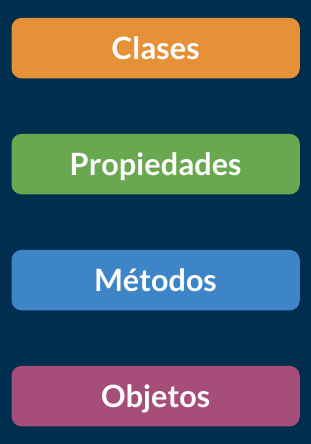
\includegraphics[scale=0.45]{./Pictures/001_poo_elementos.png}
\end{figure}

Además, se basa en los siguientes 4 pilares:\\

\begin{figure}[h!]
  \centering
  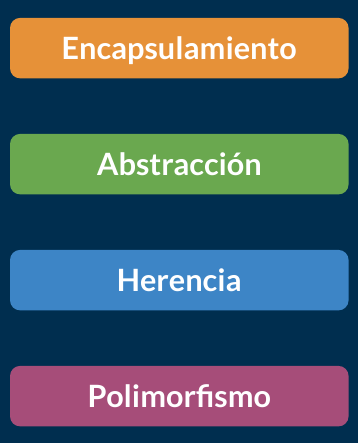
\includegraphics[scale=0.45]{./Pictures/002_pilares_POO.png}
\end{figure}

La programación Oritentada a objetos también tiene mucho que ver con
\textbf{UML Unified Modeling Language}.\\

\begin{figure}[h!]
  \centering
  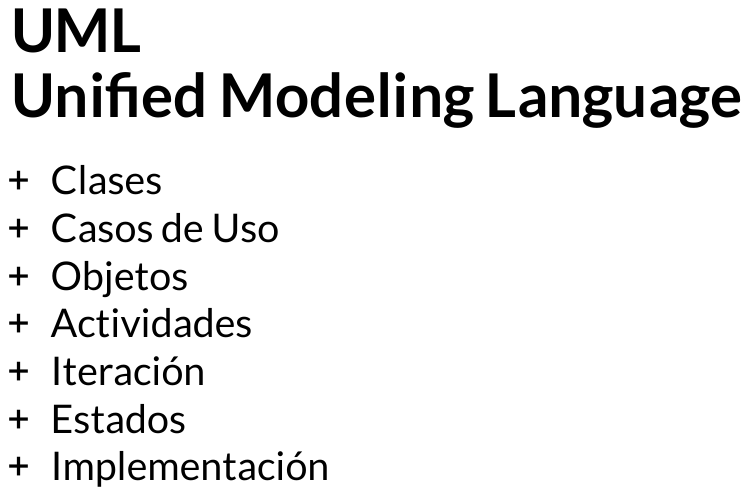
\includegraphics[scale=0.4]{./Pictures/003_uml.png}
\end{figure}

%% Clase 2
\section{¿Qué es un Objeto?}%
Los \textbf{Objetos} son todas las cosas físicas o conceptuales que tienen
propiedades y comportamientos. Por ejemplo: usuario (fisico), sesion
(conceptual), auto, etc.\\

\begin{figure}[h!]
  \centering
  
\includegraphics[scale=0.45]{./Pictures/004_objetos.png}
\end{figure}

Las \textbf{Propiedades} o atributos son las características de nuestro
objetos. Estos atributos siempre serán sustantivos y pueden tener diferentes
valores que harán referencia a nombres, tamaños, formas y estados.\\

Por ejemplo: el color de auto es verde o rojo (\texttt{color} es el atributo,
\texttt{verde} y \texttt{rojo} son posibles valores para este atributo).\\

Los\textbf{Comportamientos} o métodos serán todas las operaciones de nuestros
objetos que solemos llamar usando verbos o sustantivos y verbos. Por ejemplo
los métodos del objeto sesión pueden ser \texttt{login()}, \texttt{logout()},
\texttt{makeReport()}, etc.


%% Clase 3
\section{Abstracción: ¿Qué es una Clase?}%
La \textbf{Abstracción} se trata de analizar objetos de forma independiente, sus
propiedades, características y comportamientos, para abstraer su composición y
generar un modelo, lo que traducimos a código como clases.\\

\begin{figure}[h!]
  \centering
  
\includegraphics[scale=0.5]{./Pictures/005_clases_objetos.png}
\end{figure}

Las \textbf{Clases} son los modelos sobre los cuales construimos nuestros
objetos, es decir, las clases son los “moldes” que nos permiten generar
objetos. Cada clase debe tener identidad (con un nombre de clase único usando
Upper Camel Case), estado (con sus atributos) y comportamiento (con sus métodos
y operaciones).\\

Una vez ya tenemos lo suficiente abstracción de un objeto podemos representar
las clases usando UML.\\

\begin{figure}[h!]
  \centering
  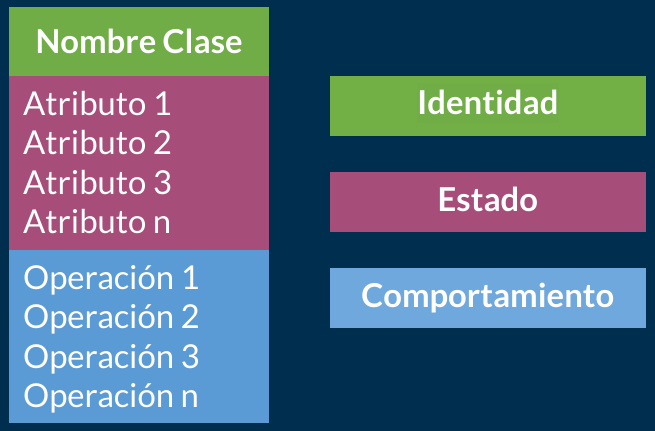
\includegraphics[scale=0.5]{./Pictures/006_uml.png}
\end{figure}

Por ejemplo:\\

El ejemplo de clase más típico en Internet:\\

\begin{figure}[h!]
  \centering
  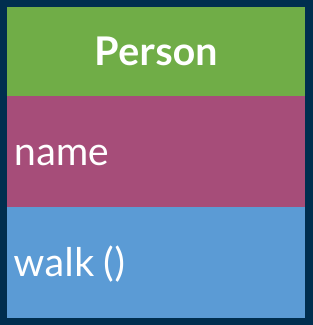
\includegraphics[scale=0.5]{./Pictures/007_clase_person.png}
\end{figure}


%% Clase 4
\section{Modularidad}%
La \textbf{Modularidad} consiste en dividir nuestro programa en diferentes módulos de
forma que puedan unirse o separarse sin romperse entre ellos o perder alguna
funcionalidad.\\

\begin{figure}[h!]
  \centering
  
\includegraphics[scale=0.7]{./Pictures/008_modularidad.png}
\end{figure}

La Modularidad en Programación Orientada a Objetos nos ayuda a:\\

\begin{itemize}
  \item Reutilizar código.
  \item Evitar colapsos.
  \item Que nuestro código sea mantenible.
  \item Mejorar la legibilidad.
  \item Resolución rápida de problemas.
\end{itemize}

Es recomendable separar los módulos en diferentes archivos. En general cada
archivo tiene una clase y si bien es cierto hay ocasiones en las que en un
archivo hay varias clases, esto es la excepción y no la norma.\\

%% Clase 5
\section{Creando nuestra primera Clase}%
Nuestro proyecto en este curso es construir un sistema que nos permita listar y
agendar nuestras citas médicas, por lo que debemos crear algunas clases para
cada integrante del sistema: doctores, pacientes, entre otras.\\

Así vamos a crear nuestra primer clase con sus métodos y atributos:\\

\textbf{Main.java}
\begin{minted}{java}
  public class Main {
      public static void main(String[] args) {

      }
  }
\end{minted}

\textbf{Doctor.java}
\begin{minted}{java}
  public class doctor {
      int id;
      string name;
      string speciality;

      // comportamientos
      public void showname() {
          system.out.println(name);
      }
  }
\end{minted}

Perfecto, ya tenemos nuestra primera clase creada. Ahora veamos lo que podemos
hacer con esta clase. Vamos hablar como podemos utilizar esto:\\

Declarando un objeto:\\
\begin{figure}[h!]
  \centering
  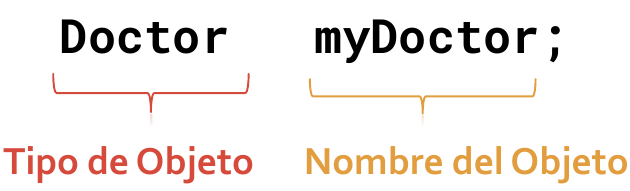
\includegraphics[scale=0.35]{./Pictures/009_declarar_objetos.png}
\end{figure}

Instanciando un objeto:\\
\begin{figure}[h!]
  \centering
  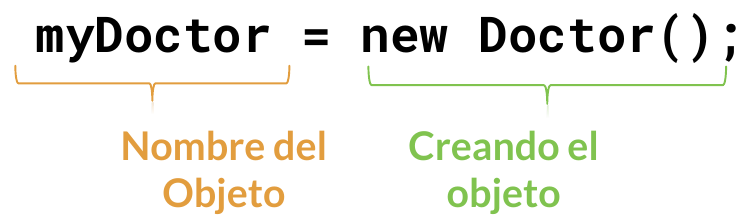
\includegraphics[scale=0.35]{./Pictures/010_instanciar_objetos.png}
\end{figure}

Declarando e instanciando un objeto:
\begin{figure}[h!]
  \centering
  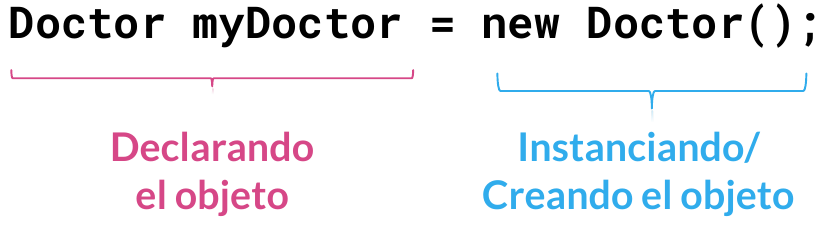
\includegraphics[scale=0.35]{./Pictures/011_dec_instan.png}
\end{figure}

Veamos como se haría en nuestro proyecto:\\

\textbf{Main.java}
\begin{minted}{java}
  public class Main {
      public static void main(String[] args) {

          Doctor myDoctor = new Doctor();
          myDoctor.name = "Alejandro Rodríguez";
          myDoctor.showName();
      }
  }
\end{minted}

\begin{figure}[h!]
  \centering
  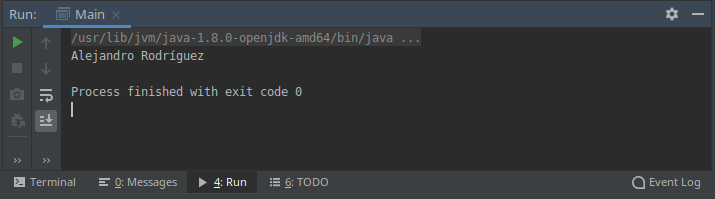
\includegraphics[scale=0.75]{./Pictures/013_primer_objeto.png}
\end{figure}


%% Clase 6
\section{Método constructor}%
El Método Constructor es el primer método que se ejecuta por defecto cuando
creamos una clase, nos permite crear nuevas instancias de una clase. Lo
invocamos con la palabra reservada new seguida del nombre con el que
inicializamos la clase y paréntesis.\\

\begin{figure}[h!]
  \centering
  
\includegraphics[scale=0.35]{./Pictures/012_met_constructor.png}
\end{figure}

El compilador de Java crea un método constructor en caso de que no definamos
uno, pero de todas formas es muy buena idea programarlo nosotros, ya que nos
permite definir y/o configurar el comportamiento de nuestros objetos usando
argumentos.\\

El método constructor no debe regresar ningún valor (no necesitamos un return).
Más adelante estudiaremos un poco más a fondo cómo funcionan la sobrecarga de
métodos y sobrecarga de constructores.\\

\textbf{Doctor.java}
\begin{minted}{java}
  public class Doctor {
      int id;
      String name;
      String speciality;

      Doctor() {
          System.out.println("Construyendo el Objeto Doctor");
      }

      // Comportamientos
      public void showName() {
          System.out.println(name);
      }
  }
\end{minted}

\begin{figure}[h!]
  \centering
  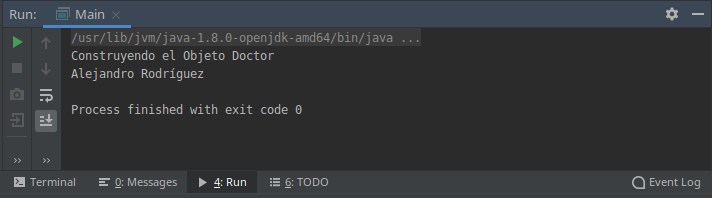
\includegraphics[scale=0.75]{./Pictures/014_constructor.png}
\end{figure}

\textbf{Main.java}
\begin{minted}{java}
  public class Main {
      public static void main(String[] args) {

          Doctor myDoctor = new Doctor("Ahahí Salgado");
          myDoctor.name = "Alejandro Rodríguez";
          myDoctor.showName();
      }
  }
\end{minted}

\textbf{Doctor.java}
\begin{minted}{java}
  public class Doctor {
      int id;
      String name;
      String speciality;

      Doctor() {
          System.out.println("Construyendo el Objeto Doctor");
      }

      Doctor(String name) {
          System.out.println("El nombre del Doctor asignado es: " + name);
      }

      // Comportamientos
      public void showName() {
          System.out.println(name);
      }
  }
\end{minted}

Hemos definido un constructor que acepta un String como argumento:\\

\begin{figure}[h!]
  \centering
  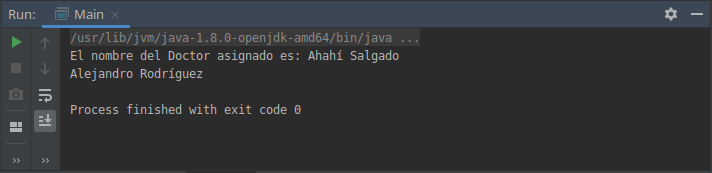
\includegraphics[scale=0.75]{./Pictures/015_constructor.png}
\end{figure}




%% Clase 7
\section{Static: Variables y Métodos Estáticos}%
Los métodos y variables estáticos nos ayudan a ejecutar o conseguir algún
código desde clases que no han sido instanciadas, ya que sus valores se guardan
en la memoria de nuestro programa, no en diferentes objetos instanciados a
través de una clase.\\

Por ejemplo:
\begin{minted}{java}
  public class Calculadora {
      public static int suma(int a, int b) {
          return a + b;
      }
  }
\end{minted}

Podemos invocar al método suma sin necesidad de instanciar un objeto:
\begin{minted}{java}
    Calculadora.suma(5,2);
\end{minted}

También funciona con variables estáticas:

\begin{minted}{java}
  public class Calculadora {
      public static final double PI = 3.1415926;
      public static int valor = 0;
  }
\end{minted}

Y éstas se podrían usar de la siguiente manera;

\begin{minted}{java}
  Calculadora.PI;
  Calculadora.valor;
\end{minted}


Las variables estáticas mantienen su valor durante todo el ciclo de vida de
nuestro programa, por lo tanto, podemos alterar los valores de una variable
estática desde una clase y consumir su valor alterado desde otra sin necesidad
de conectar ambas clases.\\

También podemos importar los métodos estáticos de una clase para usarlos sin
necesidad de escribir el nombre de la clase:\\

\begin{minted}{java}
  import static com.anncode.operaciones.Calculadora.*
  import static java.lang.Math.*

  public clas Principal {
      public static void (String[] args) {
          int number = suma(3, 5);
          System.out.println(number + PI);
      }
  }
\end{minted}


%% Clase 8
\section{Creando elementos estáticos}%
En muchos casos nuestro código necesita ejecutar métodos que no necesariamente
deben pertenecer a un objeto o instancia en concreto, ya que pueden ser muy
generales (así como Math.Random) o los valores que almacenamos deben ser los
mismos, sin importar si los consumimos desde una o más clases.\\

En todos estos casos vale la pena usar variables y métodos estáticos.\\

Por ejemplo en nuestra clase Doctor el atributo id debe ser autoincrementado
por naturaleza. Por eso pondremos nuestra variablde id como static:\\

\textbf{Doctor.java}
\begin{minted}{java}
  public class Doctor {
      // Atributos
      static int id = 0;   // Autoincrement
      String name;
      String speciality;

      Doctor() {
          System.out.println("Construyendo el Objeto Doctor");
          id++;
      }

      Doctor(String name) {
          System.out.println("El nombre del Doctor asignado es: " + name);
      }

      // Comportamientos
      public void showName() {
          System.out.println(name);
      }

      public void showId() {
          System.out.println("ID Doctor: " + id);
      }
  }
\end{minted}


\textbf{Main.java}
\begin{minted}{java}
  public class Main {
      public static void main(String[] args) {

          Doctor myDoctor = new Doctor();
          myDoctor.name = "Alejandro Rodríguez";
          myDoctor.showName();
          myDoctor.showId();
          System.out.println(Doctor.id);

          Doctor myDoctorAnn = new Doctor();
          myDoctorAnn.showId();
          System.out.println(Doctor.id);
      }
  }
\end{minted}

\begin{figure}[h!]
  \centering
  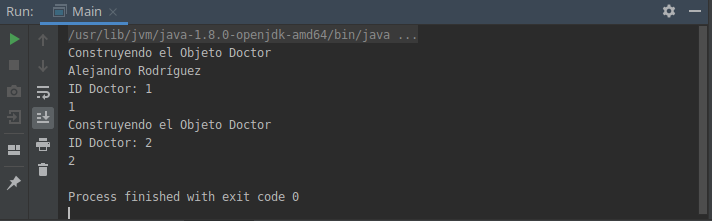
\includegraphics[scale=0.75]{./Pictures/016_static_id.png}
\end{figure}

También podemos manipular la variable estática \textbf{id} de la clase
\textbf{Doctor} desde otras clases por ejemplo desde la clase \textbf{Main}:\\

\textbf{Main.java}
\begin{minted}{java}
  public class Main {
      public static void main(String[] args) {

          Doctor myDoctor = new Doctor();
          myDoctor.name = "Alejandro Rodríguez";
          myDoctor.showName();
          myDoctor.showId();
          System.out.println(Doctor.id);

          Doctor.id++;

          Doctor myDoctorAnn = new Doctor();
          myDoctorAnn.showId();
          System.out.println(Doctor.id);
      }
  }
\end{minted}

\begin{figure}[h!]
  \centering
  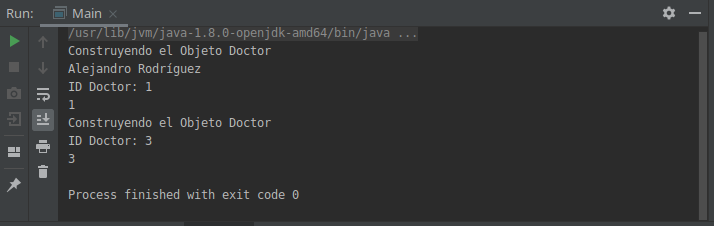
\includegraphics[scale=0.75]{./Pictures/017_static_id.png}
\end{figure}

Con lo aprendido de los métodos státicos vamos a crear una interfaz de usuario
simple en una nueva clase llamada \textbf{UIMenu}\\

\textbf{UIMenu.java}
\begin{minted}{java}
  import java.util.Scanner;

  public class UIMenu {

      public static void showMenu() {
          System.out.println("Welcome to My Appointments");
          System.out.println("Selecciona la acción deseada");

          int response = 0;
          do {
              System.out.println("1. Doctor");
              System.out.println("2. Patient");
              System.out.println("0. Salir");

              Scanner sc = new Scanner(System.in);
              response = Integer.valueOf(sc.nextLine());


              switch (response) {
                  case 1:
                      System.out.println("Doctor");
                      break;
                  case 2:
                      response = 0;
                      showPatientMenu();
                      break;
                  case 0:
                      System.out.println("Thank you for you visit.");
                      break;
                  default:
                      System.out.println("Please select a correct answer.");
              }
          } while (response != 0);
      }

      public static void showPatientMenu() {
          int response = 0;
          do {
              System.out.println("\n\n");
              System.out.println("Patient");
              System.out.println("1. Book an appointment");
              System.out.println("2. My appointments");
              System.out.println("0. Return");

              Scanner sc = new Scanner(System.in);
              response = Integer.valueOf(sc.nextLine());

              switch (response) {
                  case 1:
                      System.out.println("::Book an appointment");
                      break;
                  case 2:
                      System.out.println("::My appointments");
                      break;
                  case 0:
                      showMenu();
                      break;
              }
          } while (response != 0);
      }
  }
\end{minted}

\textbf{Main.java}
\begin{minted}{java}
  public class Main {
      public static void main(String[] args) {

          Doctor myDoctor = new Doctor();
          myDoctor.name = "Alejandro Rodríguez";
          myDoctor.showName();
          myDoctor.showId();

          Doctor myDoctorAnn = new Doctor();
          myDoctorAnn.showId();

          UIMenu.showMenu();
      }
  }
\end{minted}

\newpage

\begin{figure}[h!]
  \centering
  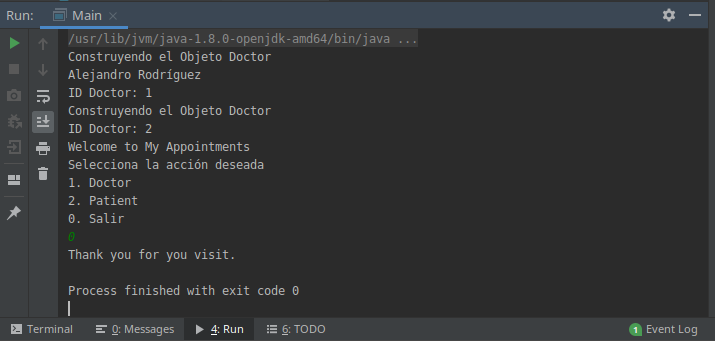
\includegraphics[scale=0.75]{./Pictures/018_static_proyecto.png}
\end{figure}

También podemos aprovechar la sintaxis de \textbf{import} para llamar al método
estático \textbf{showMenu()} sin la necesidad de mencionar a \textbf{UIMenu}.\\

Para esto creamos el paquete ui:

\begin{figure}[h!]
  \centering
  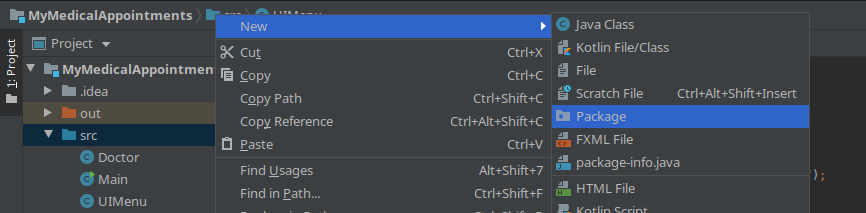
\includegraphics[scale=0.75]{./Pictures/019_package.png}
\end{figure}

\begin{figure}[h!]
  \centering
  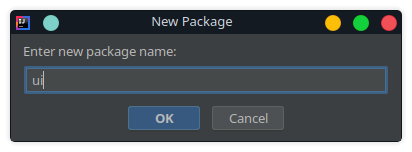
\includegraphics[scale=0.75]{./Pictures/020_nombre_package.png}
\end{figure}

Luego movemos la clase \textbf{UIMenu} dentro de la carpeta \textbf{ui} y
refactorizamos como se ve en la siguientes imágenes:

\begin{figure}[h!]
  \centering
  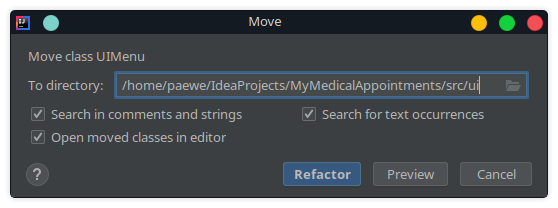
\includegraphics[scale=0.75]{./Pictures/021_move_UIMenu.png}
\end{figure}

\begin{figure}[h!]
  \centering
  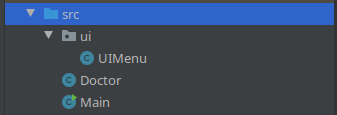
\includegraphics[scale=0.75]{./Pictures/022_package_ui.png}
\end{figure}

Al refactorizar, nótese como en la parte superior de la clase \textbf{UIMenu}
aparece la palabra clave \textbf{package} con el nombre del paquete que en este
caso es \textbf{ui}.\\

\begin{figure}[h!]
  \centering
  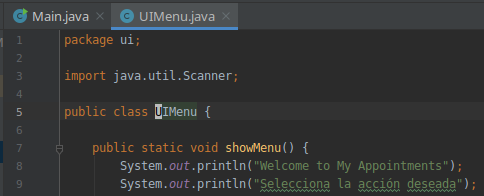
\includegraphics[scale=0.75]{./Pictures/023_package_ui.png}
\end{figure}

De igual manera en la clase \textbf{Main} aparece la palabra clave
\textbf{import} que nos permite usar el método \textbf{showMenu()} del paquete
\textbf{ui}.\\

\begin{figure}[h!]
  \centering
  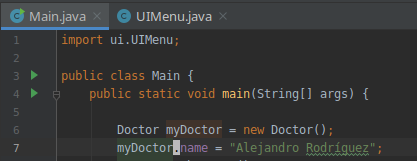
\includegraphics[scale=0.75]{./Pictures/024_package_main.png}
\end{figure}

Pero nosotros vamos a importar el método estático para poder usarlo sin tener
que mencionar a la clase UIMenu:\\

\textbf{UIMenu.java}
\begin{minted}{java}
  package ui;

  import java.util.Scanner;

  public class UIMenu {

      public static void showMenu() {
          System.out.println("Welcome to My Appointments");
          System.out.println("Selecciona la acción deseada");

          int response = 0;
          do {
              System.out.println("1. Doctor");
              System.out.println("2. Patient");
              System.out.println("0. Salir");

              Scanner sc = new Scanner(System.in);
              response = Integer.valueOf(sc.nextLine());


              switch (response) {
                  case 1:
                      System.out.println("Doctor");
                      break;
                  case 2:
                      response = 0;
                      showPatientMenu();
                      break;
                  case 0:
                      System.out.println("Thank you for you visit.");
                      break;
                  default:
                      System.out.println("Please select a correct answer.");
              }
          } while (response != 0);
      }

      public static void showPatientMenu() {
          int response = 0;
          do {
              System.out.println("\n\n");
              System.out.println("Patient");
              System.out.println("1. Book an appointment");
              System.out.println("2. My appointments");
              System.out.println("0. Return");

              Scanner sc = new Scanner(System.in);
              response = Integer.valueOf(sc.nextLine());

              switch (response) {
                  case 1:
                      System.out.println("::Book an appointment");
                      break;
                  case 2:
                      System.out.println("::My appointments");
                      break;
                  case 0:
                      showMenu();
                      break;
              }
          } while (response != 0);
      }
  }
\end{minted}

\textbf{Nota:} Para que el scope (alcance) del método \textbf{showMenu()} nos
permita utilizarlo en nuestra clase Main entonces delante del método debe
figurar la palabra clave \textbf{public}.\\

\textbf{Main.java}
\begin{minted}{java}
  import static ui.UIMenu.*;

  public class Main {
      public static void main(String[] args) {

          Doctor myDoctor = new Doctor();
          myDoctor.name = "Alejandro Rodríguez";
          myDoctor.showName();
          myDoctor.showId();

          Doctor myDoctorAnn = new Doctor();
          myDoctorAnn.showId();

          showMenu();
      }
  }
\end{minted}

\begin{figure}[h!]
  \centering
  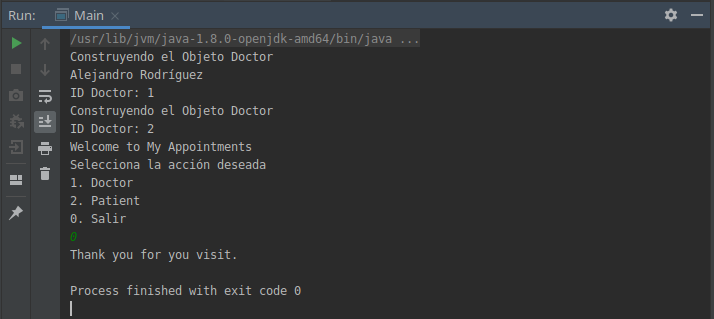
\includegraphics[scale=0.75]{./Pictures/025_resultados.png}
\end{figure}


%% Clase 9
\section{Final: Variables Constantes}%
Para definir una variable constante se usa la palabra reservada \textbf{final}, por ejemplo:

\begin{minted}{java}
  public class Calculadora {
    public static final double PI = 3.1415926;
  }
\end{minted}

Y podemos usar esta variable de la siguiente manera:

\begin{minted}{java}
  Calculadora.PI;
\end{minted}

Ahora vamos aplicar esto en el proyecto, ya que crearemos una variable estática
y constante \textbf{MONTHS} con los meses del año y se desplegará en el menú,
veamos:\\

\textbf{UIMenu.java}
\begin{minted}{java}
  package ui;

  import java.util.Scanner;

  public class UIMenu {

      public static final String[] MONTHS = {
          "Enero", "Febrero", "Marzo", "Abril", "Mayo", "Junio",
          "Julio", "Agosto", "Setiembre", "Octubre", "Noviembre", "Diciembre"
      };

      public static void showMenu() {
          System.out.println("Welcome to My Appointments");
          System.out.println("Selecciona la acción deseada");

          int response = 0;
          do {
              System.out.println("1. Doctor");
              System.out.println("2. Patient");
              System.out.println("0. Salir");

              Scanner sc = new Scanner(System.in);
              response = Integer.valueOf(sc.nextLine());


              switch (response) {
                  case 1:
                      System.out.println("Doctor");
                      break;
                  case 2:
                      response = 0;
                      showPatientMenu();
                      break;
                  case 0:
                      System.out.println("Thank you for you visit.");
                      break;
                  default:
                      System.out.println("Please select a correct answer.");
              }
          } while (response != 0);
      }

      public static void showPatientMenu() {
          int response = 0;
          do {
              System.out.println("\n\n");
              System.out.println("Patient");
              System.out.println("1. Book an appointment");
              System.out.println("2. My appointments");
              System.out.println("0. Return");

              Scanner sc = new Scanner(System.in);
              response = Integer.valueOf(sc.nextLine());

              switch (response) {
                  case 1:
                      System.out.println("::Book an appointment");
                      for (int i = 0; i < 3; i++) {
                          System.out.println(i + ". " + MONTHS[i]);
                      }
                      break;
                  case 2:
                      System.out.println("::My appointments");
                      break;
                  case 0:
                      showMenu();
                      break;
              }
          } while (response != 0);
      }
  }
\end{minted}


\textbf{Main.java}
\begin{minted}{java}
  import static ui.UIMenu.*;

  public class Main {
      public static void main(String[] args) {

          showMenu();
      }
  }
\end{minted}

El resultado que obtendremos se verá así:
\begin{figure}[h!]
  \centering
  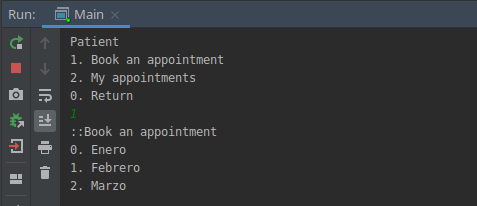
\includegraphics[scale=0.75]{./Pictures/026_resultado_c9.png}
\end{figure}


%% Clase 11
\section{¡Reto!}%
Ahora estás listo para resolver tu primer reto que en realidad es muy sencillo
de hacer.\\

Mira el siguiente diagrama y construye la clase Patient.\\

Patient\\
name: String\\
email:String\\
address: String\\
phoneNumber: String\\
birthday: String\\
weight: double\\
height: double\\
blood: String\\
Patient(name: String, email: String)\\


\begin{minted}{java}
  public class Patient {
    String name;
    String email;
    String address;
    String phoneNumber;
    String birthday;
    double weight;
    double height;
    String blood;

    public Patient(String name, String email) {
      this.name = name;
      this.email = email;
    }
  }
\end{minted}



%% Clase 10
\section{Variable vs. Objeto: Un vistazo a la memoria}%
Un objeto es una referencia a un espacio en memoria. Cuando creamos objetos,
Java los guarda en la memoria y nos devuelve coordenadas con las que podremos
acceder a la información que almacenamos.\\

Existen dos tipos de memoria: Stack y Heap.\\

La memoria Stack es mucho más rápida y nos permite almacenar nuestra
información de forma “ordenada”. Aquí se guardan las variables y sus valores de
tipos de datos primitivos (booleanos, números, strings, entre otros).\\

Los objetos también usan la memoria Stack, pero no para guardar su información,
sino para guardar las coordenadas a la verdadera ubicación del objeto en la
memoria Heap, una memoria que nos permite guardar grandes cantidades de
información, pero con un poco menos de velocidad.\\

\begin{figure}[h!]
  \centering
  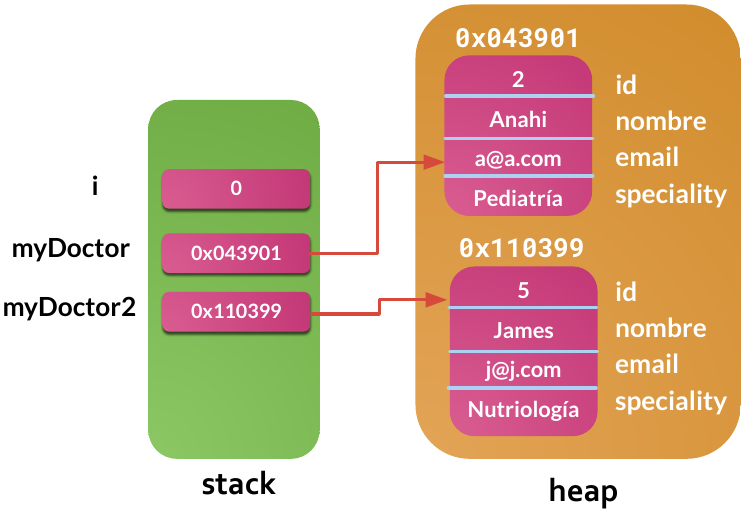
\includegraphics[scale=0.5]{./Pictures/027_var_vs_objeto.png}
\end{figure}

Veamos un ejemplo:

\begin{minted}{java}
  import static ui.UIMenu.*;

  public class Main {
      public static void main(String[] args) {

          Patient patient = new Patient("Alejandra", "alejandra@mail.com");
          Patient patient2 = new Patient("Anahi", "anahi@mail.com");

          System.out.println(patient.name);
          System.out.println(patient2.name);
          patient2 = patient;

          System.out.println(patient.name);
          System.out.println(patient2.name);

          patient2.name = "Manuel";
          System.out.println(patient.name);
          System.out.println(patient2.name);
      }
  }
\end{minted}




%% Clase 12
\section{Sobrecarga de métodos y constructores}%
A veces necesitamos que dos o más métodos de una misma clase tengan el mismo
nombre, pero con diferentes argumentos o distintos tipos de argumentos/valores
de retorno.\\

Afortunadamente, Java nos permite ejecutar código y métodos diferentes
dependiendo de los argumentos que reciba nuestra clase.\\

El uso más común de la sobrecarga de métodos es la sobrecarga de constructores
para instanciar objetos de formas distintas dependiendo de la cantidad de
argumentos que enviamos.\\

\textbf{Calculadora.java}
\begin{minted}{java}
  public class Calculadora {
      public int suma(int a, int b) {
          return a + b;
      }

      public float suma(float a, float b) {
          return a + b;
      }

      public float suma(int a, float b) {
          return a + b;
      }
  }
\end{minted}

Por ejemplo en nuestro proyecto apliquemos sobrecarga en nuestro constructor Doctor:

\textbf{Doctor.java}
\begin{minted}{java}
  public class Doctor {
      // Atributos
      static int id = 0;   // Autoincrement
      String name;
      String speciality;

      Doctor() {
          System.out.println("Construyendo el Objeto Doctor");
      }

      Doctor(String name, String speciality) {
          System.out.println("El nombre  " + name);
          id++;
          this.name = name;
          this.speciality = speciality;
      }

      // Comportamientos
      public void showName() {
          System.out.println(name);
      }

      public void showId() {
          System.out.println("ID Doctor: " + id);
      }
  }
\end{minted}

\textbf{Main.java}
\begin{minted}{java}
  import static ui.UIMenu.*;

  public class Main {
      public static void main(String[] args) {

          Doctor myDoctor = new Doctor("Anahí Salgado", "Pediatría");
          System.out.println(myDoctor.name);
          System.out.println(myDoctor.speciality);
      }
  }
\end{minted}

\begin{figure}[h!]
  \centering
  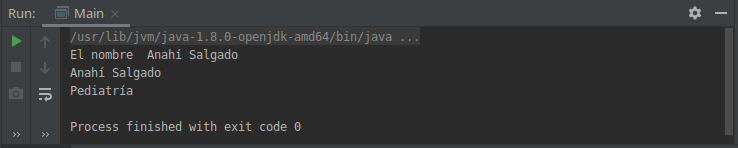
\includegraphics[scale=0.75]{./Pictures/029_sobrecarga_constructor.png}
\end{figure}


%% Clase 13
\section{Encapsulamiento: Modificadores de acceso}%
Los Modificadores de Acceso nos ayudan a limitar desde dónde podemos leer o
modificar atributos especiales de nuestras clases. Podemos definir qué
variables se pueden leer/editar por fuera de las clases donde fueron creadas.
Esto lo conocemos como Encapsulamiento.\\

\textbf{Patient.java}
\begin{minted}{java}
  public class Patient {
      // Atributos
      String name;
      String email;
      String address;
      String phoneNumber;
      String birthday;
      double weight;
      double height;
      String blood;

      Patient(String name, String email) {
          this.name = name;
          this.email = email;
      }
  }
\end{minted}

\textbf{Main.java}
\begin{minted}{java}
  import static ui.UIMenu.*;

  public class Main {
      public static void main(String[] args) {

          Doctor myDoctor = new Doctor("Anahí Salgado", "Pediatría");
          System.out.println(myDoctor.name);
          System.out.println(myDoctor.speciality);

          Patient patient = new Patient("Alejandra", "alejandra@mail.com");
          System.out.println(patient.name);
          System.out.println(patient.email);

          patient.weight = 60.5;  // kg   Genera incosistencia
          patient.height = 1.65;  // Mts  Genera incosistencia

          System.out.println(patient.weight); // Genera incosistencia
          System.out.println(patient.height); // Genera incosistencia

          patient.weight = 54.5; // Genera incosistencia
          patient.name = "Juan"; // Genera incosistencia
      }
  }
\end{minted}

Para evitar estas inconsistencias está el \textbf{encapsulamiento}. Para esto
podemos utilizar los modificadores de acceso:\\

\begin{figure}[h!]
  \centering
  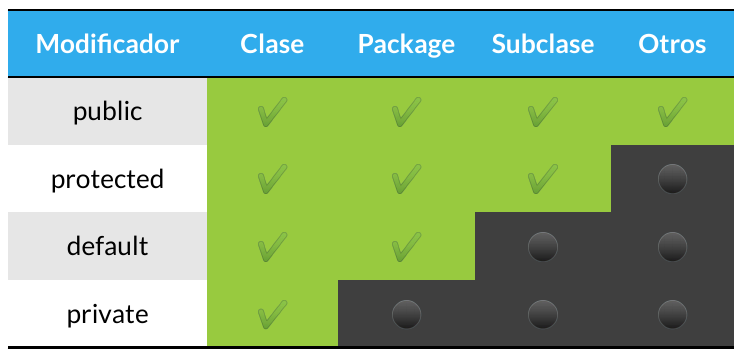
\includegraphics[scale=0.5]{./Pictures/030_mod_acceso.png}
\end{figure}

Vamos a modificar nuestros atributos de la clase \textbf{Patient} con los
modificadores de acceso.\\

\textbf{Patient.java}
\begin{minted}{java}
  public class Patient {
      // Atributos
      private String name;
      private String email;
      private String address;
      private String phoneNumber;
      private String birthday;
      private double weight;
      private double height;
      String blood;

      Patient(String name, String email) {
          this.name = name;
          this.email = email;
          this.weight = 54.5;
          System.out.println(weight + "kg.");
      }
  }
\end{minted}

\textbf{Main.java}
\begin{minted}{java}
  import static ui.UIMenu.*;

  public class Main {
      public static void main(String[] args) {

          Doctor myDoctor = new Doctor("Anahí Salgado", "Pediatría");
          System.out.println(myDoctor.name);
          System.out.println(myDoctor.speciality);

          Patient patient = new Patient("Alejandra", "alejandra@mail.com");
      }
  }
\end{minted}

\begin{figure}[h!]
  \centering
  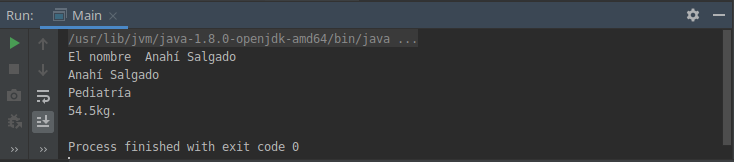
\includegraphics[scale=0.75]{./Pictures/031_resultado_encaps.png}
\end{figure}



\newpage
%% Clase 14
\section{Getters y Setters}%
Los Getters y Setters nos permiten leer y escribir (respectivamente) los
valores de nuestras variables privadas desde fuera de la clase donde fueron
creadas. Con los Getters obtenemos los datos de las variables y con los Setters
asignamos o cambiamos su valor.\\

También puedes usar los atajos de tu IDE favorito para generar los métodos
getters y setters de todas o algunas de tus variables.\\

\begin{figure}[h!]
  \centering
  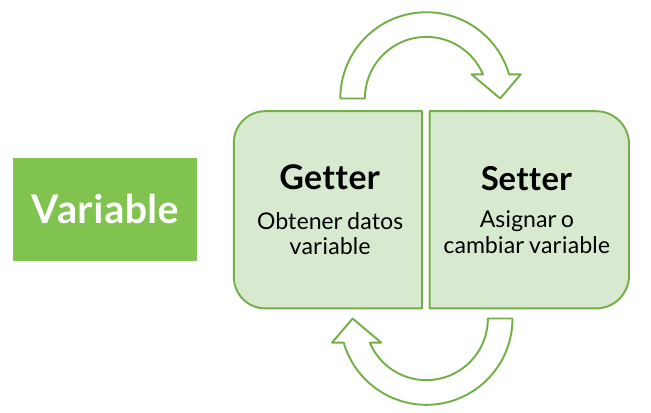
\includegraphics[scale=0.5]{./Pictures/032_get_set.png}
\end{figure}

\textbf{Patient.java}
\begin{minted}{java}
public class Patient {
    // Atributos
    private String name;
    private String email;
    private String address;
    private String phoneNumber;
    private String birthday;
    private double weight;
    private double height;
    String blood;

    Patient(String name, String email) {
        this.name = name;
        this.email = email;
        this.weight = 54.5;
        System.out.println(weight + "kg.");
    }

    public void setWeight(double weight) {
        this.weight = weight;
    }

    public String getWeight() {
        return weight + " Kg.";
    }
}
\end{minted}

También podemos usar la herramienta que nos proporciona IntelliJ IDEA para
generar automáticamente el código.\\

\newpage
Clic derecho - Generate - Getter and Setter - OK\\

\begin{figure}[h!]
  \centering
  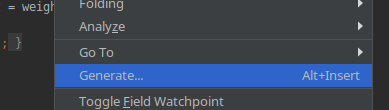
\includegraphics[scale=0.75]{./Pictures/033_generate.png}
\end{figure}

\begin{figure}[h!]
  \centering
  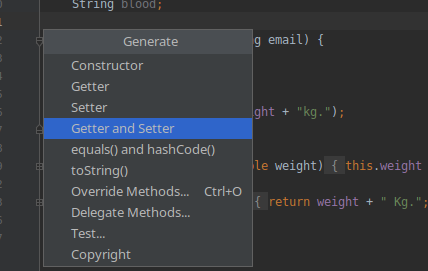
\includegraphics[scale=0.75]{./Pictures/034_generate.png}
\end{figure}

\begin{figure}[h!]
  \centering
  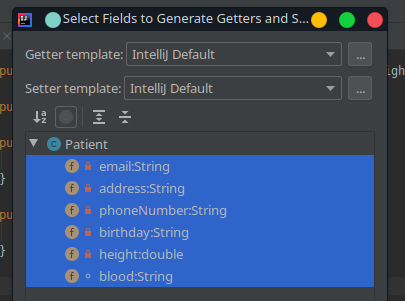
\includegraphics[scale=0.75]{./Pictures/035_generate.png}
\end{figure}

Luego de esto se generarán los getters y setters para cada uno de nuestros
atributos.\\


\textbf{Patient.java}
\begin{minted}{java}
  public class Patient {
      // Atributos
      private String name;
      private String email;
      private String address;
      private String phoneNumber;
      private String birthday;
      private double weight;
      private double height;
      String blood;

      Patient(String name, String email) {
          this.name = name;
          this.email = email;
          this.weight = 54.5;
          System.out.println(weight + "kg.");
      }

      public void setWeight(double weight) {
          this.weight = weight;
      }

      public String getWeight() {
          return weight + " Kg.";
      }

      public String getName() {
          return name;
      }

      public void setName(String name) {
          this.name = name;
      }

      public String getEmail() {
          return email;
      }

      public void setEmail(String email) {
          this.email = email;
      }

      public String getAddress() {
          return address;
      }

      public void setAddress(String address) {
          this.address = address;
      }

      public String getPhoneNumber() {
          return phoneNumber;
      }

      public void setPhoneNumber(String phoneNumber) {
          if (phoneNumber.length() > 8) {
              System.out.println("El nro telefónico debe ser de 8 dígitos máximo");
          } else if (phoneNumber.length() == 8) {
              this.phoneNumber = phoneNumber;
          }
      }

      public String getBirthday() {
          return birthday;
      }

      public void setBirthday(String birthday) {
          this.birthday = birthday;
      }

      public String getHeight() {
          return height + " Mts.";
      }

      public void setHeight(double height) {
          this.height = height;
      }

      public String getBlood() {
          return blood;
      }

      public void setBlood(String blood) {
          this.blood = blood;
      }
  }
\end{minted}

\textbf{Main.java}
\begin{minted}{java}
  import static ui.UIMenu.*;

  public class Main {
      public static void main(String[] args) {

          Doctor myDoctor = new Doctor("Anahí Salgado", "Pediatría");
          System.out.println(myDoctor.name);
          System.out.println(myDoctor.speciality);

          Patient patient = new Patient("Alejandra", "alejandra@mail.com");
          patient.setWeight(54.6);
          System.out.println(patient.getWeight());

          patient.setPhoneNumber("123456789");
          System.out.println(patient.getPhoneNumber());
      }
  }
\end{minted}

\begin{figure}[h!]
  \centering
  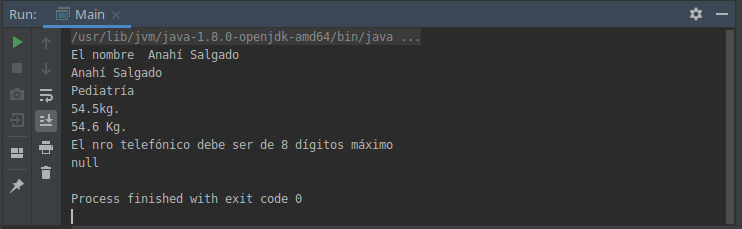
\includegraphics[scale=0.75]{./Pictures/036_set_get.png}
\end{figure}

\newpage

Ahora en cambio si seteamos el phoneNumber con 8 dígitos, cumpliendo nuestra
condición entonces:\\

\textbf{Main.java}
\begin{minted}{java}
  import static ui.UIMenu.*;

  public class Main {
      public static void main(String[] args) {

          Doctor myDoctor = new Doctor("Anahí Salgado", "Pediatría");
          System.out.println(myDoctor.name);
          System.out.println(myDoctor.speciality);

          Patient patient = new Patient("Alejandra", "alejandra@mail.com");
          patient.setWeight(54.6);
          System.out.println(patient.getWeight());

          patient.setPhoneNumber("12345678");
          System.out.println(patient.getPhoneNumber());
      }
  }
\end{minted}

\begin{figure}[h!]
  \centering
  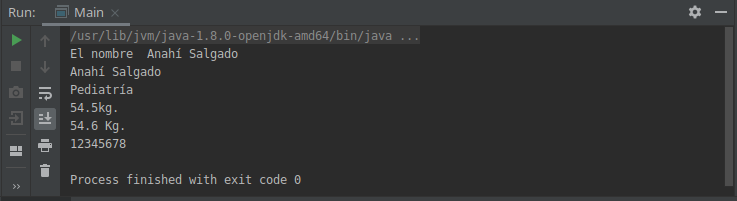
\includegraphics[scale=0.75]{./Pictures/037_set_get.png}
\end{figure}


%% Clase 15
\section{Variable vs. Objeto}%
Las Variables son entidades elementales muy sencillas, pueden ser números,
caracteres, booleanos, entre otras. Los Objetos son entidades complejas que
pueden estar formadas por la agrupación de diferentes variables y métodos.\\

Los Objetos Primitivos o Clases Wrapper son variables primitivas que trabajan
con algún tipo de dato y también tienen las características de los objetos.\\

\begin{figure}[h!]
  \centering
  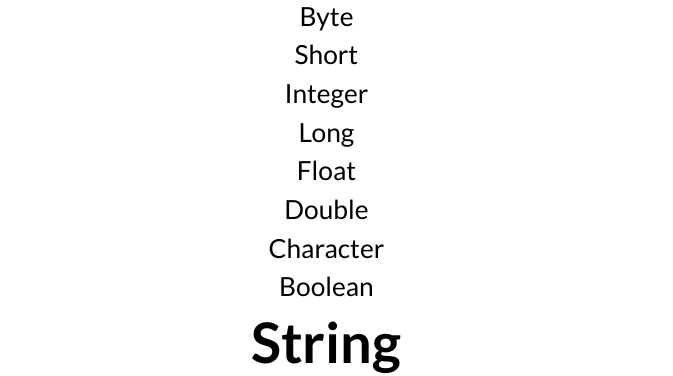
\includegraphics[scale=0.5]{./Pictures/038_class_wrapper.png}
\end{figure}


%% Clase 16
\section{Clases Anidadas}%
Las Clases Anidadas o Clases Helper son clases dentro de otras clases que
agrupamos por su lógica y/o características en común.\\

Podemos encontrar clases estáticas anidadas, clases internas que son locales a
un método o clases internas anónimas. Las clases anidadas pueden llamar a
cualquier tipo de elemento o método de nuestras clases.\\

\begin{figure}[h!]
  \centering
  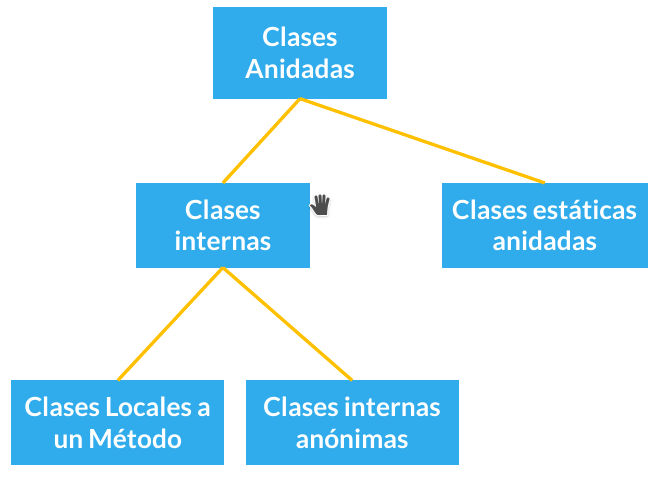
\includegraphics[scale=0.5]{./Pictures/039_clases_anidadas.png}
\end{figure}

Las clases internas anónimas se verán más a detenimiento en el curso de Java
Orientado a la programación funcional.

Las Clases Estáticas no necesitan ser instanciadas para poder ser llamadas y
ejecutadas, aunque debes recordar que solo permiten llamar a los métodos
estáticos de sus clases padre.\\

\begin{minted}{java}
  class ClaseExterior {
    static class ClaseStaticaAnidada {

    }

    class ClaseInterna {

    }
  }
\end{minted}

Las clases estáticas anidadas no necesitan crear instancias para llamarlas.

\begin{minted}{java}
  public class Enclosing {
    private static int x = 1;

    public static class StaticNested {
      private void run() {
        // implementacion
      }
    }
  }

  public class Main {
    public static void main(String[] args) {
      Enclosing.StaticNested nested = new Enclosing.StaticNested();
      nested.run();
    }
  }
\end{minted}


\textbf{Doctor.java}
\begin{minted}{java}
  import java.util.ArrayList;
  import java.util.Date;

  public class Doctor {
      // Atributos
      static int id = 0;   // Autoincrement
      private String name;
      private String email;
      private String speciality;

      Doctor() {
          System.out.println("Construyendo el Objeto Doctor");
      }

      Doctor(String name, String speciality) {
          System.out.println("El nombre  " + name);
          id++;
          this.name = name;
          this.speciality = speciality;
      }

      // Comportamientos
      public void showName() {
          System.out.println(name);
      }

      public void showId() {
          System.out.println("ID Doctor: " + id);
      }

      ArrayList<AvailableAppointment> availableAppointments = new ArrayList<>();
      public void addAvailableAppointment(Date date, String time) {
          availableAppointments.add(new Doctor.AvailableAppointment(date, time));
      }

      public ArrayList<AvailableAppointment> getAvailableAppointments() {
          return availableAppointments;
      }

      public static class AvailableAppointment {
          private int id;
          private Date date;
          private String time;

          public AvailableAppointment(Date date, String time) {
              this.date = date;
              this.time = time;
          }

          public int getId() {
              return id;
          }

          public void setId(int id) {
              this.id = id;
          }

          public Date getDate() {
              return date;
          }

          public void setDate(Date date) {
              this.date = date;
          }

          public String getTime() {
              return time;
          }

          public void setTime(String time) {
              this.time = time;
          }
      }
  }
\end{minted}

\textbf{Main.java}
\begin{minted}{java}
  import java.util.Date;

  import static ui.UIMenu.*;

  public class Main {
      public static void main(String[] args) {

          Doctor myDoctor = new Doctor("Anahí Salgado", "Pediatría");
          myDoctor.addAvailableAppointment(new Date(), "4pm");
          myDoctor.addAvailableAppointment(new Date(), "10pm");
          myDoctor.addAvailableAppointment(new Date(), "1pm");

          System.out.println(myDoctor.getAvailableAppointments());

          /*
          Patient patient = new Patient("Alejandra", "alejandra@mail.com");
          patient.setWeight(54.6);
          System.out.println(patient.getWeight());

          patient.setPhoneNumber("12345678");
          System.out.println(patient.getPhoneNumber());

          */
      }
  }
\end{minted}

\begin{figure}[h!]
  \centering
  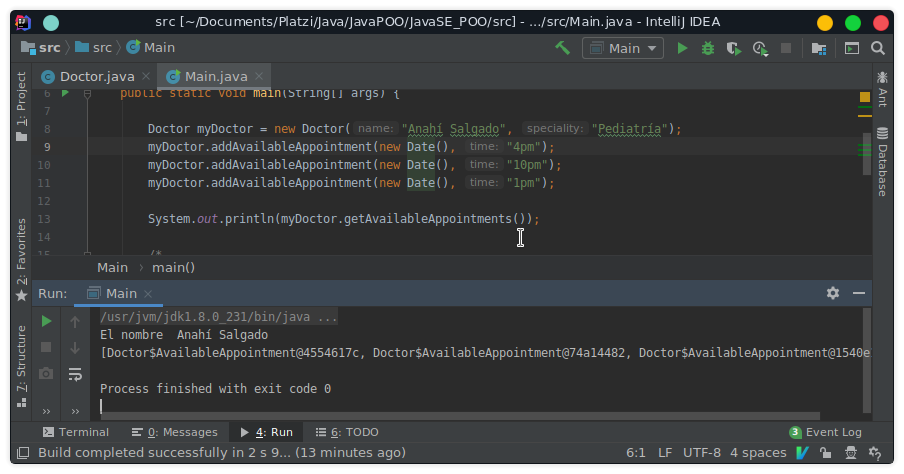
\includegraphics[scale=0.5]{./Pictures/040_clases_anidadas.png}
\end{figure}

Como se muestra al ejecutar el programa devuelve toda la lista de objetos.
Ahora como solo se quiere imprimir las citas disponibles, entonces para eso
podemos hacer un  \textbf{foreach}.\\

\textbf{Main.java}
\begin{minted}{java}
  import java.util.Date;

  import static ui.UIMenu.*;

  public class Main {
      public static void main(String[] args) {

          Doctor myDoctor = new Doctor("Anahí Salgado", "Pediatría");
          myDoctor.addAvailableAppointment(new Date(), "4pm");
          myDoctor.addAvailableAppointment(new Date(), "10pm");
          myDoctor.addAvailableAppointment(new Date(), "1pm");

          System.out.println(myDoctor.getAvailableAppointments());

          for (Doctor.AvailableAppointment aA: myDoctor.getAvailableAppointments()) {
              System.out.println(aA.getDate() + " " + aA.getTime());
          }

          /*
          Patient patient = new Patient("Alejandra", "alejandra@mail.com");
          patient.setWeight(54.6);
          System.out.println(patient.getWeight());

          patient.setPhoneNumber("12345678");
          System.out.println(patient.getPhoneNumber());

          */
      }
  }
\end{minted}

\begin{figure}[h!]
  \centering
  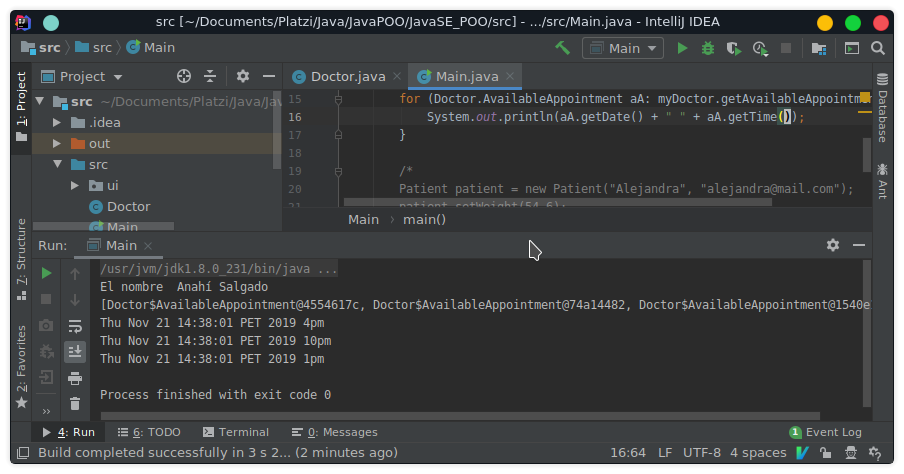
\includegraphics[scale=0.5]{./Pictures/041_foreach.png}
\end{figure}

%% Clase 17
\section{Clases Internas y Locales a un método}%

Veamos las clases internas:\\

\begin{minted}{java}
  public class Outer {
    public class Inner {

    }
  }

  public class Main {
    public static void main(String[] args) {
      Outer outer = new Outer();
      Outer.Inner inner = outer.new Inner();
    }
  }
\end{minted}

Ahora veamos las clases locales a un Método:\\


\begin{minted}{java}
  public class Enclosing {
    void run() {
      class Local {
        void run() {

        }
      }

      Local local = new Local();
      local.run();
    }
  }

  public class Main {
    public static void main(String[] args) {
      Enclosing enclosing = new Enclosing();
      enclosing.run();
    }
  }

\end{minted}

En este punto es conveniente usar las clases estáticas ya que al no necesitar
instanciarse los objetos ocupan menos espacio en la memoria.\\


%% Clase 18
\section{Enumerations}%
Los enumerations son tipos de datos muy especiales pues este, es el único en su
tipo que sirve para declarar una colección de constantes, al ser así estaremos
obligados a escribirlos con mayúsculas.\\

Usaremos enum cada vez que necesitemos representar un conjunto fijo de
constantes. Por ejemplo los días de la semana.\\

Así podemos declarar un enumeration usando la palabra reservada enum.\\

\begin{minted}{java}
  public enum Day {
    SUNDAY, MONDAY, TUESDAY, WEDNESDAY,
    THURSDAY, FRIDAY, SATURDAY
  }
\end{minted}

Puedo crear referencias de enumerations de la siguiente forma:\\

\begin{minted}{java}
  Day day;
  switch (day) {
    case MONDAY:
      System.out.println("Mondays are good.");
      break;
    case FRIDAY:
      System.out.println("Fridays are nice");
      break;
    case SATURDAY: case: SUNDAY:
      System.out.println("Weekends are the best");
      break;
    default:
      System.out.println("Midweek are so-so");
      break;
  }
\end{minted}

Y puedo llamar un valor del enumeration así:\\

\begin{minted}{java}
  Day.MONDAY;
  Day.FRIDAY;
  Day.SATURDAY
\end{minted}

Los enumerations pueden tener atributos, métodos y constructores, como se
muestra:\\

\begin{minted}{java}
  public enum Day {
    MONDAY("Lunes");
    TUESDAY("Jueves");
    FRIDAY("Viernes");
    SATURDAY("Sábado");
    SUNDAY("Domingo");

    private String spanish;
    private Day(String s) {
      spanish = s;
    }

    private String getSpanish() {
      return spanish;
    }
  }
\end{minted}

Y para utilizarlo lo podemos hacer así:\\

\begin{minted}{java}
  System.out.println(Day.MONDAY);
\end{minted}

Imprimirá: MONDAY\\

\begin{minted}{java}
  System.out.println(Day.MONDAY.getSpanish());
\end{minted}

Imprimirá: Lunes\\


%% Clase 19
\section{¿Qué es la Herencia? Don't repeat Yourself}%
Don’t repeat yourself (DRY) consiste en detectar cuando estamos repitiendo el
mismo código una y otra vez para crear algún método o función que nos ayude a
evitar estos repetidos.\\

Esta es una de las bases de la programación que siempre debemos tener en
cuenta, ya que nos ayuda a reducir la dificultad de nuestro código para
implementar cambios y/o mejoras en nuestra aplicación.\\

La Herencia consiste en crear nuevas clases a partir de otras clases,
establecemos una relación padre e hijo entre nuestras clases. Es diferente a
las clases anidadas, ya que, en vez de crear clases dentro de clases, le
indicamos a nuestras subclases de qué superclase pueden heredar (extends) para
reutilizar el código de algunos de sus métodos.\\

Recuerda que nuestras clases no pueden heredar de más de una clase.\\

\begin{minted}{java}
  public class SuperClass {
      // ...
  }

  public class SubClass extends SuperClass {
      // ...
  }
\end{minted}


%% Clase 20
\section{Super y This}%
\textbf{Super} indica que una variable o método es de la clase padre, la
superclase de cual heredan nuestras subclases, solo la usamos cuando aplicamos
herencia.\\

Además, podemos llamar al constructor de la clase padre desde sus diferentes
subclases usando super(); y enviando los argumentos que sean necesarios.\\

Por otro lado, this nos permite especificar que nuestras variables están
señalando a la misma clase donde estamos trabajando, ya sea una clase normal,
anidada, subclase o superclase.\\

\begin{minted}{java}
  public class User {
    int age = 1;

    public int getAge() {
      return this.age;
    }
  }

  public class Doctor extends User {
    String speciality = "Dentist";

    Doctor() {
      super.getAge(); // 1
      this.getSpeciality(); // Dentist
    }

    public int getSpeciality() {
      return this.speciality;
    }
  }
\end{minted}


\textbf{User.java}
\begin{minted}{java}
  public class User {
      private int id;
      private String name;
      private String email;
      private String address;
      private String phoneNumber;

      public User(String name, String email) {
          this.name = name;
          this.email = email;
      }

      public int getId() {
          return id;
      }

      public void setId(int id) {
          this.id = id;
      }

      public String getName() {
          return name;
      }

      public void setName(String name) {
          this.name = name;
      }

      public String getEmail() {
          return email;
      }

      public void setEmail(String email) {
          this.email = email;
      }

      public String getAddress() {
          return address;
      }

      public void setAddress(String address) {
          this.address = address;
      }

      public String getPhoneNumber() {
          return phoneNumber;
      }

      public void setPhoneNumber(String phoneNumber) {
          if (phoneNumber.length() > 8) {
              System.out.println("El nro telefónico debe ser de 8 dígitos máximo");
          } else if (phoneNumber.length() == 8) {
              this.phoneNumber = phoneNumber;
          }
      }
  }
\end{minted}

\textbf{Doctor.java}
\begin{minted}{java}
  import java.util.ArrayList;
  import java.util.Date;

  public class Doctor extends User {
      // Atributo
      private String speciality;

      Doctor(String name, String email) {
          super(name, email);
      }

      public String getSpeciality() {
          return speciality;
      }

      public void setSpeciality(String speciality) {
          this.speciality = speciality;
      }

      public void setAvailableAppointments(ArrayList<AvailableAppointment> availableAppointments) {
          this.availableAppointments = availableAppointments;
      }

      ArrayList<AvailableAppointment> availableAppointments = new ArrayList<>();
      public void addAvailableAppointment(Date date, String time) {
          availableAppointments.add(new Doctor.AvailableAppointment(date, time));
      }

      public ArrayList<AvailableAppointment> getAvailableAppointments() {
          return availableAppointments;
      }

      public static class AvailableAppointment {
          private int id;
          private Date date;
          private String time;

          public AvailableAppointment(Date date, String time) {
              this.date = date;
              this.time = time;
          }

          public Date getDate() {
              return date;
          }

          public void setDate(Date date) {
              this.date = date;
          }

          public String getTime() {
              return time;
          }

          public void setTime(String time) {
              this.time = time;
          }
      }
  }
\end{minted}

\textbf{Patient.java}
\begin{minted}{java}
  public class Patient extends User {
      // Atributos
      private String birthday;
      private double weight;
      private double height;
      String blood;

      Patient(String name, String email) {
          super(name, email);
      }

      public void setWeight(double weight) {
          this.weight = weight;
      }

      public String getWeight() {
          return weight + " Kg.";
      }

  }
\end{minted}


\begin{figure}[h!]
  \centering
  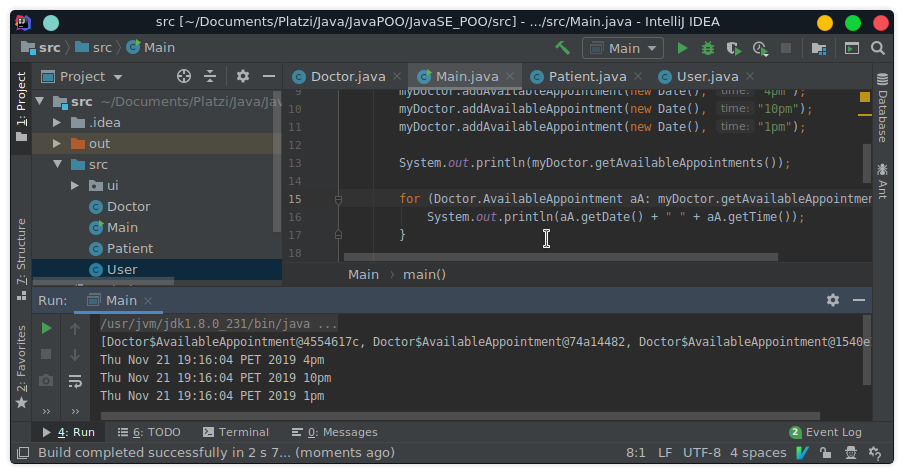
\includegraphics[scale=0.5]{./Pictures/042_herencia.png}
\end{figure}

Vemos como a pesar de haber refactorizado nuestro código nuestra aplicación aún
sigue funcionando.\\

\textbf{Nota: En Java no se permite la herencia múltiple.}


%% Clase 21
\section{Polimorfismo: Sobreescritura de Métodos}%
El Polimorfismo es una característica de la programación orientada a objetos
que consiste en sobrescribir algunos métodos de la clase de la cual heredan
nuestras subclases para asignar comportamientos diferentes.\\

Además de los métodos de las superclases, también podemos redefinir el
comportamiento de los métodos que “heredan” todos nuestros objetos, así como
.toString, hashCode, finalize, notify, entre otros.\\

La sobreescritura de constructores consiste en usar los miembros heredados de
una supreclase pero con argumentos diferentes.\\

\textbf{User.java}
\begin{minted}{java}
  public class User {
      private int id;
      private String name;
      private String email;
      private String address;
      private String phoneNumber;

      public User(String name, String email) {
          this.name = name;
          this.email = email;
      }

      public int getId() {
          return id;
      }

      public void setId(int id) {
          this.id = id;
      }

      public String getName() {
          return name;
      }

      public void setName(String name) {
          this.name = name;
      }

      public String getEmail() {
          return email;
      }

      public void setEmail(String email) {
          this.email = email;
      }

      public String getAddress() {
          return address;
      }

      public void setAddress(String address) {
          this.address = address;
      }

      public String getPhoneNumber() {
          return phoneNumber;
      }

      public void setPhoneNumber(String phoneNumber) {
          if (phoneNumber.length() > 8) {
              System.out.println("El nro telefónico debe ser de 8 dígitos máximo");
          } else if (phoneNumber.length() == 8) {
              this.phoneNumber = phoneNumber;
          }
      }

      @Override
      public String toString() {
          return "User: " + name + ", Email: " + email  +
          "\nAddress: " + address + ". Phone: " + phoneNumber;
      }
  }
\end{minted}

\begin{figure}[h!]
  \centering
  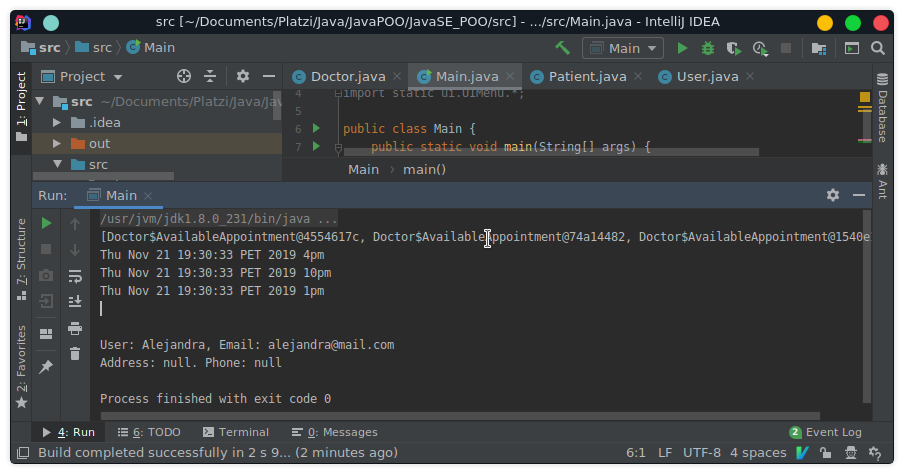
\includegraphics[scale=0.5]{./Pictures/043_polimorfirmo.png}
\end{figure}

\textbf{Patient.java}
\begin{minted}{java}
  public class Patient extends User {
      // Atributos
      private String birthday;
      private double weight;
      private double height;
      String blood;

      Patient(String name, String email) {
          super(name, email);
          // mas instrucciones
      }

      public void setWeight(double weight) {
          this.weight = weight;
      }

      public String getWeight() {
          return weight + " Kg.";
      }

      public void setHeight(double height) {
          this.height = height;
      }

      public String getHeight() {
          return height + " Kg.";
      }

      @Override
      public String toString() {
          return super.toString() + "\nAge: " + birthday + "\n Weight: " + getWeight() +
                  "\n Height:" + getHeight() + "\nBlood: " + blood;
      }
  }
\end{minted}

\textbf{Main.java}
\begin{minted}{java}
  import java.util.Date;

  import static ui.UIMenu.*;

  public class Main {
      public static void main(String[] args) {

          Doctor myDoctor = new Doctor("Anahí Salgado", "Pediatría");
          myDoctor.addAvailableAppointment(new Date(), "4pm");
          myDoctor.addAvailableAppointment(new Date(), "10pm");
          myDoctor.addAvailableAppointment(new Date(), "1pm");

          System.out.println(myDoctor.getAvailableAppointments());

          for (Doctor.AvailableAppointment aA: myDoctor.getAvailableAppointments()) {
              System.out.println(aA.getDate() + " " + aA.getTime());
          }

          System.out.println();
          System.out.println();
          Patient patient = new Patient("Alejandra", "alejandra@mail.com");
          System.out.println(patient);
      }
  }
\end{minted}

\begin{figure}[h!]
  \centering
  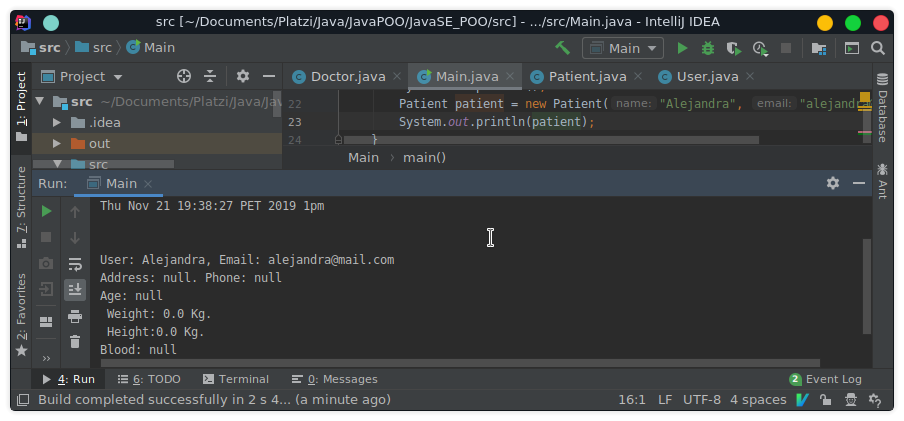
\includegraphics[scale=0.5]{./Pictures/044_polimorfismo.png}
\end{figure}


Recuerda que no podemos sobrescribir los métodos marcados como final o
static.\\


%% Clase 22
\section{Polimorfismo: Sobreescribiendo el método toString}%
Recuerda que el método toString viene heredada de la clase Object. Todas las
clases heredan de Object.\\

\textbf{Doctor.java}
\begin{minted}{java}
  import java.util.ArrayList;
  import java.util.Date;

  public class Doctor extends User {
      // Atributo
      private String speciality;

      Doctor(String name, String email) {
          super(name, email);
      }

      public String getSpeciality() {
          return speciality;
      }

      public void setSpeciality(String speciality) {
          this.speciality = speciality;
      }

      public void setAvailableAppointments(ArrayList<AvailableAppointment> availableAppointments) {
          this.availableAppointments = availableAppointments;
      }

      ArrayList<AvailableAppointment> availableAppointments = new ArrayList<>();
      public void addAvailableAppointment(Date date, String time) {
          availableAppointments.add(new Doctor.AvailableAppointment(date, time));
      }

      public ArrayList<AvailableAppointment> getAvailableAppointments() {
          return availableAppointments;
      }

      @Override
      public String toString() {
          return super.toString() + "\nSpeciality: " + speciality +
          "\nAvailable: " + availableAppointments.toString();
      }

      public static class AvailableAppointment {
          private int id;
          private Date date;
          private String time;

          public AvailableAppointment(Date date, String time) {
              this.date = date;
              this.time = time;
          }

          public Date getDate() {
              return date;
          }

          public void setDate(Date date) {
              this.date = date;
          }

          public String getTime() {
              return time;
          }

          public void setTime(String time) {
              this.time = time;
          }

          @Override
          public String toString() {
              return "Available Appointments \nDate: " + date + "\nTime: " + time;
          }
      }
  }
\end{minted}

\textbf{Main.java}
\begin{minted}{java}
  import java.sql.SQLOutput;
  import java.util.Date;

  import static ui.UIMenu.*;

  public class Main {
      public static void main(String[] args) {

          Doctor myDoctor = new Doctor("Anahí Salgado", "anahi@anahi.com");
          myDoctor.addAvailableAppointment(new Date(), "4pm");
          myDoctor.addAvailableAppointment(new Date(), "10pm");
          myDoctor.addAvailableAppointment(new Date(), "1pm");

          /*
          System.out.println(myDoctor.getAvailableAppointments());

          for (Doctor.AvailableAppointment aA: myDoctor.getAvailableAppointments()) {
              System.out.println(aA.getDate() + " " + aA.getTime());
          }
          */

          System.out.println(myDoctor);

          System.out.println();
          System.out.println();
          Patient patient = new Patient("Alejandra", "alejandra@mail.com");
          System.out.println(patient);
      }
  }
\end{minted}

\newpage

\begin{figure}[h!]
  \centering
  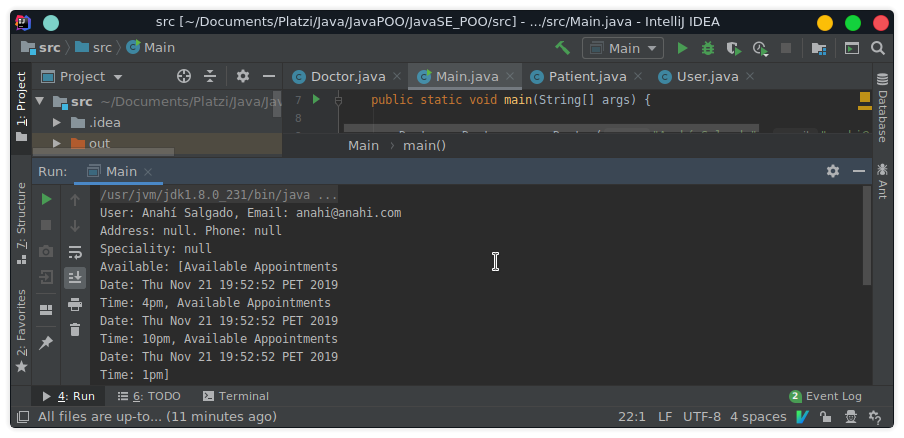
\includegraphics[scale=0.5]{./Pictures/045_toString.png}
\end{figure}


%% Clase 23
\section{Interfaces}%

\begin{figure}[h!]
  \centering
  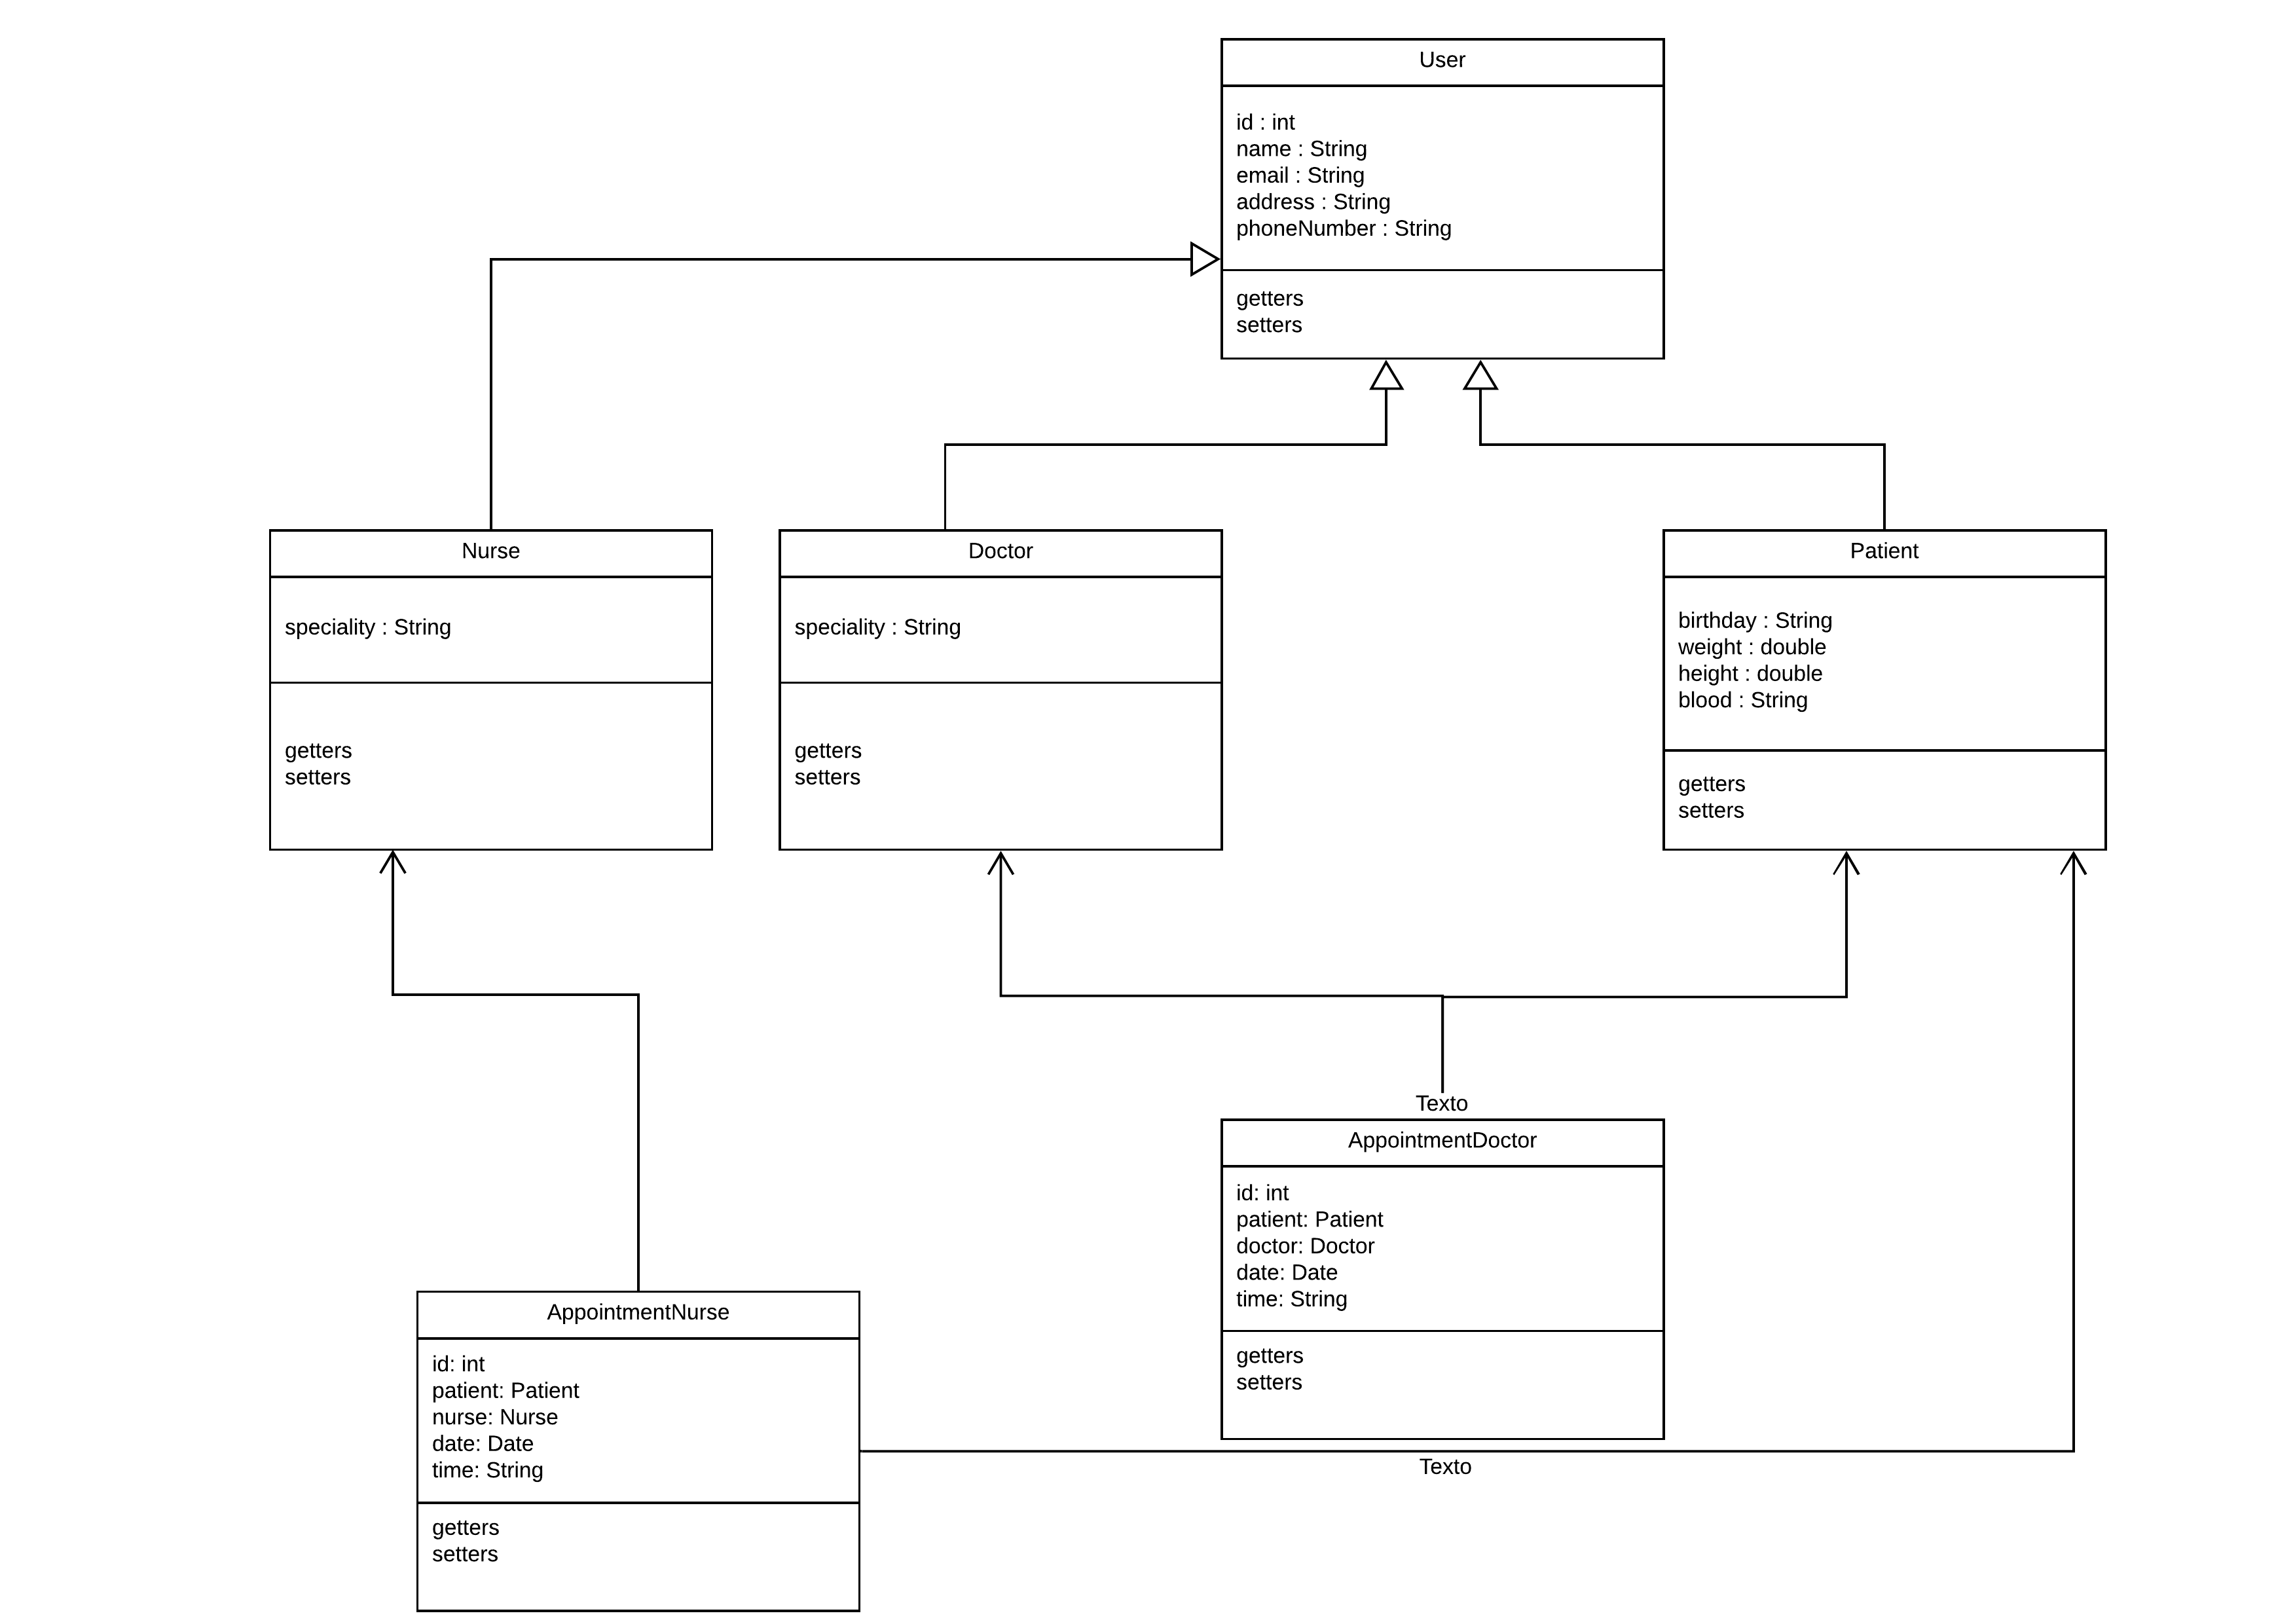
\includegraphics[scale=0.5]{./Pictures/046_diagrama.png}
\end{figure}

Las Interfaces son un tipo de referencia similar a una clase con solo
constantes y definiciones de métodos, son de gran ayuda para definir los
comportamientos que son redundantes y queremos reutilizar un más de una clase,
incluso cuando tenemos muchas clases y no todas pertenecen a la misma
“familia”.\\

Las interfaces establecen la forma de las clases que la implementan, así como
sus nombres de métodos, listas de argumentos y listas de retorno, pero NO sus
bloques de código, eso es responsabilidad de cada clase.\\


%% Clase 24
\section{Creando una interfaz para definir si una fecha es agendable}%
Composición de Interfaces en Clases: abstraer todos los métodos/comportamientos
de una clase para modularizarlos (comprimirlos, encapsularlos) en una interfaz
y reutilizar su código en diferentes clases.\\

Las interfaces se crean utilizando la palabra reservada interface y se
implementan en nuestras clases con implements.\\

Recuerda que podemos heredar (implementar) más de una interfaz, pero no podemos
hacerlo de las clases padres o superclases.\\

\textbf{Model/AppointmentDoctor.java}
\begin{minted}{java}
  package Model;

  import java.util.Date;

  public class AppointmentDoctor implements ISchedulable {
      private int id;
      private Patient patient;
      private Doctor doctor;
      private Date date;
      private String time;

      public int getId() {
          return id;
      }

      public void setId(int id) {
          this.id = id;
      }

      public Patient getPatient() {
          return patient;
      }

      public void setPatient(Patient patient) {
          this.patient = patient;
      }

      public Doctor getDoctor() {
          return doctor;
      }

      public void setDoctor(Doctor doctor) {
          this.doctor = doctor;
      }

      public Date getDate() {
          return date;
      }

      public void setDate(Date date) {
          this.date = date;
      }

      public String getTime() {
          return time;
      }

      public void setTime(String time) {
          this.time = time;
      }

      @Override
      public void schedule(Date date, String time) {

      }
  }
\end{minted}

\textbf{Model/Nurse.java}
\begin{minted}{java}
  package Model;

  public class Nurse extends User {

      private String speciality;

      public Nurse(String name, String email) {
          super(name, email);
      }

      public String getSpeciality() {
          return speciality;
      }

      public void setSpeciality(String speciality) {
          this.speciality = speciality;
      }
  }
\end{minted}

\textbf{Model/AppointmentNurse.java}
\begin{minted}{java}
  package Model;

  import java.util.Date;

  public class AppointmentNurse implements ISchedulable {
      private int id;
      private Nurse nurse;
      private Patient patient;
      private Date date;
      private String time;

      public int getId() {
          return id;
      }

      public void setId(int id) {
          this.id = id;
      }

      public Nurse getNurse() {
          return nurse;
      }

      public void setNurse(Nurse nurse) {
          this.nurse = nurse;
      }

      public Patient getPatient() {
          return patient;
      }

      public void setPatient(Patient patient) {
          this.patient = patient;
      }

      public Date getDate() {
          return date;
      }

      public void setDate(Date date) {
          this.date = date;
      }

      public String getTime() {
          return time;
      }

      public void setTime(String time) {
          this.time = time;
      }

      @Override
      public void schedule(Date date, String time) {

      }
  }
\end{minted}

\textbf{ISchedulable.java}
\begin{minted}{java}
  package Model;

  import java.util.Date;

  public interface ISchedulable {

      void schedule(Date date, String time);
  }
\end{minted}

\textbf{Main.java}
\begin{minted}{java}
  import Model.Doctor;
  import Model.Patient;

  import java.util.Date;

  public class Main {
      public static void main(String[] args) {

          Doctor myDoctor = new Doctor("Anahí Salgado", "anahi@anahi.com");
          myDoctor.addAvailableAppointment(new Date(), "4pm");
          myDoctor.addAvailableAppointment(new Date(), "10pm");
          myDoctor.addAvailableAppointment(new Date(), "1pm");

          /*
          System.out.println(myDoctor.getAvailableAppointments());

          for (Model.Doctor.AvailableAppointment aA: myDoctor.getAvailableAppointments()) {
              System.out.println(aA.getDate() + " " + aA.getTime());
          }
          */

          System.out.println(myDoctor);

          System.out.println();
          System.out.println();
          Patient patient = new Patient("Alejandra", "alejandra@mail.com");
          System.out.println(patient);
      }
  }
\end{minted}




%% Clase 25
\section{Collections}%
Otras interfaces que son muy importantes en Java son los llamados Collections\\

Los Collections nos van a servir para trabajar con colecciones de datos,
específicamente y solamente con objetos, para esto recuerda que tenemos
disponibles nuestras clases Wrapper que nos ayudan a convertir datos primitivos
a objetos.\\

Los collections se diferencian de los arrays en que su tamaño no es fijo y por
el contrario es dinámico.\\

A continuación te muestro un diagrama de su composición:\\

\textbf{Imagen}\\

Como podemos observar el elemento más alto es la interfaz Collection, para lo
cual, partiendo de su naturalidad de interface, entendemos que tiene una serie
de métodos “básicos” dónde su comportamiento será definido a medida que se vaya
implementando en más elementos. De ella se desprenden principalmente las
interfaces Set y List.\\

La interface Set tendrá las siguientes características:\\

Almacena objetos únicos, no repetidos.\\
La mayoría de las veces los objetos se almacenarán en desorden.\\
No tenemos índice.\\

La interface List tiene éstas características:\\

Puede almacenar objetos repetidos.\\
Los objetos se almacenan en orden secuencial.\\
Tenemos acceso al índice.\\

\subsection*{Si seguimos analizando las familias tenemos que de Set se desprenden:}%
Clase HashSet\\
Interfaz SortedSet y de ella la clase TreeSet.\\

HashSet los elementos se guardan en desorden y gracias al mecanismo llamado
hashing (obtiene un identificador del objeto) permite almacenar objetos únicos.\\

TreeSet almacena objetos únicos, y gracias a su estructura de árbol el *acceso
es sumamente rápido.\\

\subsection*{Ahora si analizamos la familia List, de ella se desprenden:}%
Clase ArrayList puede tener duplicados, no está sincronizada por lo tanto es
más rápida\\
Clase Vector es sincronizada, los datos están más seguros pero es más lento.\\
Clase LinkedList, puede contener elementos duplicados, no está sincronizada (es
más rápida) al ser una estructura de datos doblemente ligada podemos añadir
datos por encima de la pila o por debajo.\\



\textbf{Imagen}\\



\subsection*{Sigamos con Map}%
Lo primero que debes saber es que tiene tres implementaciones:\\

HashTable\\
LinkedHashMap\\
HashMap\\
SortedMap $->$ TreeMap\\



\textbf{Imagen}\\



La interfaz Map no hereda de la interfaz Collection porque representa una
estructura de datos de Mapeo y no de colección simple de objetos. Esta
estructura es más compleja, pues cada elemento deberá venir en pareja con otro
dato que funcionará como la llave del elemento.\\


\textbf{Map}\\
Donde K es el key o clave\\
Donde V es el value o valor\\

Podemos declarar un map de la siguiente forma:\\

\begin{minted}{java}
  Map<Integer, String> map = new HashMap<Integer, String>();
  Map<Integer, String> treeMap = new TreeMap<Integer, String>();
  Map<Integer, String> linkedHashMap = new LinkedHashMap<Integer, String>();
\end{minted}

Como observas solo se puede construir el objeto con tres elementos que
implementan de ella: HashMap, TreeMap y LinkedHashMap dejando fuera HashTable y
SortedMap. SortedMap estará fuera pues es una interfaz y HashTable ha quedado
deprecada pues tiene métodos redundantes en otras clases. Mira la funcionalidad
de cada uno.\\

Como te conté hace un momento Map tiene implementaciones:\\

HashMap: Los elementos no se ordenan. No aceptan claves duplicadas ni valores
nulos.\\
LinkedHashMap: Ordena los elementos conforme se van insertando; provocando que
las búsquedas sean más lentas que las demás clases.\\
TreeMap: El Mapa lo ordena de forma “natural”. Por ejemplo, si la clave son
valores enteros (como luego veremos), los ordena de menos a mayor.\\

Para iterar alguno de estos será necesario utilizar la interface Iterator y
para recorrerlo lo haremos un bucle while así como se muestra:\\

\textbf{Para HashMap}\\

\begin{minted}{java}
  // Imprimimos el Map con un Iterador
  Iterator it = map.keySet().iterator();
  while(it.hasNext()){
    Integer key = it.next();
    System.out.println("Clave: " + key + " -> Valor: " + map.get(key));
  }
\end{minted}

\textbf{Para LinkedHashMap}\\

\begin{minted}{java}
  // Imprimimos el Map con un Iterador
  Iterator it = linkedHashMap.keySet().iterator();
  while(it.hasNext()){
    Integer key = it.next();
    System.out.println("Clave: " + key + " -> Valor: " + linkedHashMap.get(key));
  }
\end{minted}

\textbf{Para TreeMap}

\begin{minted}{java}
  // Imprimimos el Map con un Iterador
  Iterator it = treeMap.keySet().iterator();
  while(it.hasNext()){
    Integer key = it.next();
    System.out.println("Clave: " + key + " -> Valor: " + treeMap.get(key));
  }
\end{minted}

Ahora lee esta lectura y en la sección de tutoriales cuéntanos en tus palabras
cómo funciona Deque.


%% Clase 26
\section{Clases Abstractas}%
A veces NO necesitamos implementar todos los métodos de una clase heredada o
interfaz. No siempre necesitamos crear instancias o implementar todos los
métodos heredados de una clase padre, así como tampoco podremos necesitamos
algún método de nuestras interfaces, pero estas nos obligan a escribir el
código de todos los métodos que definimos genéricamente.\\

Afortunadamente, las Clases Abstractas resuelven todos estos problemas. Son una
combinación entre interfaces y herencia donde no implementaremos todos los
métodos ni tampoco crearemos instancias.\\

\begin{minted}{java}
  public abstract class Figura {
    // ...
  }

  class Triangulo extends Figura {
    // ...
  }
\end{minted}

\textbf{Model/User.java}
\begin{minted}{java}
  package Model;

  public abstract class User {
      private int id;
      private String name;
      private String email;
      private String address;
      private String phoneNumber;

      public User(String name, String email) {
          this.name = name;
          this.email = email;
      }

      public int getId() {
          return id;
      }

      public void setId(int id) {
          this.id = id;
      }

      public String getName() {
          return name;
      }

      public void setName(String name) {
          this.name = name;
      }

      public String getEmail() {
          return email;
      }

      public void setEmail(String email) {
          this.email = email;
      }

      public String getAddress() {
          return address;
      }

      public void setAddress(String address) {
          this.address = address;
      }

      public String getPhoneNumber() {
          return phoneNumber;
      }

      public void setPhoneNumber(String phoneNumber) {
          if (phoneNumber.length() > 8) {
              System.out.println("El nro telefónico debe ser de 8 dígitos máximo");
          } else if (phoneNumber.length() == 8) {
              this.phoneNumber = phoneNumber;
          }
      }

      @Override
      public String toString() {
          return "Model.User: " + name + ", Email: " + email  +
          "\nAddress: " + address + ". Phone: " + phoneNumber;
      }
  }
\end{minted}


%% Clase 27
\section{Miembros abstractos}%
Los Métodos Abstractos son los métodos que debemos implementar obligatoriamente
cada vez que usemos nuestras clases abstractas, mientras que los métodos que no
sean abstractos van a ser opcionales.\\

\begin{minted}{java}
  public abstract class Figura {
    abstract void dibujar(); // obligatorio
    void dibujar3D(); // no es obligatorio
  }

  class Triangulo extends Figura {
    void dibujar() {
      // Instrucciones para dibujar el triángulo...
    }
  }
\end{minted}

Recuerda los métodos abstractos solo se pueden implementar en clases
abstractas. Y las clases abstractas no necesitan ser instanciadas para ser
implementadas.\\

\textbf{Model/User.java}
\begin{minted}{java}
  package Model;

  public abstract class User {
      private int id;
      private String name;
      private String email;
      private String address;
      private String phoneNumber;

      public User(String name, String email) {
          this.name = name;
          this.email = email;
      }

      public int getId() {
          return id;
      }

      public void setId(int id) {
          this.id = id;
      }

      public String getName() {
          return name;
      }

      public void setName(String name) {
          this.name = name;
      }

      public String getEmail() {
          return email;
      }

      public void setEmail(String email) {
          this.email = email;
      }

      public String getAddress() {
          return address;
      }

      public void setAddress(String address) {
          this.address = address;
      }

      public String getPhoneNumber() {
          return phoneNumber;
      }

      public void setPhoneNumber(String phoneNumber) {
          if (phoneNumber.length() > 8) {
              System.out.println("El nro telefónico debe ser de 8 dígitos máximo");
          } else if (phoneNumber.length() == 8) {
              this.phoneNumber = phoneNumber;
          }
      }

      @Override
      public String toString() {
          return "Model.User: " + name + ", Email: " + email  +
          "\nAddress: " + address + ". Phone: " + phoneNumber;
      }

      public abstract void showDataUser();
  }
\end{minted}

\textbf{Model/Doctor.java}
\begin{minted}{java}
  package Model;

  import java.util.ArrayList;
  import java.util.Date;

  public class Doctor extends User {
      // Atributo
      private String speciality;

      public Doctor(String name, String email) {
          super(name, email);
      }

      public String getSpeciality() {
          return speciality;
      }

      public void setSpeciality(String speciality) {
          this.speciality = speciality;
      }

      public void setAvailableAppointments(ArrayList<AvailableAppointment> availableAppointments) {
          this.availableAppointments = availableAppointments;
      }

      ArrayList<AvailableAppointment> availableAppointments = new ArrayList<>();
      public void addAvailableAppointment(Date date, String time) {
          availableAppointments.add(new Doctor.AvailableAppointment(date, time));
      }

      public ArrayList<AvailableAppointment> getAvailableAppointments() {
          return availableAppointments;
      }

      @Override
      public String toString() {
          return super.toString() + "\nSpeciality: " + speciality +
          "\nAvailable: " + availableAppointments.toString();
      }

      @Override
      public void showDataUser() {
          System.out.println("Hospital: Cruz Roja");
          System.out.println("Departamento: Cancerología");
      }

      public static class AvailableAppointment {
          private int id;
          private Date date;
          private String time;

          public AvailableAppointment(Date date, String time) {
              this.date = date;
              this.time = time;
          }

          public Date getDate() {
              return date;
          }

          public void setDate(Date date) {
              this.date = date;
          }

          public String getTime() {
              return time;
          }

          public void setTime(String time) {
              this.time = time;
          }

          @Override
          public String toString() {
              return "Available Appointments \nDate: " + date + "\nTime: " + time;
          }
      }
  }
\end{minted}

\textbf{Model/Nurse.java}
\begin{minted}{java}
  package Model;

  public class Nurse extends User {

      private String speciality;

      public Nurse(String name, String email) {
          super(name, email);
      }

      @Override
      public void showDataUser() {
          System.out.println("Hospital: Cruz Verde");
          System.out.println("Departamento: Nutriología, Pediatría");
      }

      public String getSpeciality() {
          return speciality;
      }

      public void setSpeciality(String speciality) {
          this.speciality = speciality;
      }
  }
\end{minted}

\textbf{Model/Patient.java}
\begin{minted}{java}
  package Model;

  public class Patient extends User {
      // Atributos
      private String birthday;
      private double weight;
      private double height;
      String blood;

      public Patient(String name, String email) {
          super(name, email);
          // mas instrucciones
      }

      public void setWeight(double weight) {
          this.weight = weight;
      }

      public String getWeight() {
          return weight + " Kg.";
      }

      public void setHeight(double height) {
          this.height = height;
      }

      public String getHeight() {
          return height + " Kg.";
      }

      @Override
      public String toString() {
          return super.toString() + "\nAge: " + birthday + "\n Weight: " + getWeight() +
                  "\n Height:" + getHeight() + "\nBlood: " + blood;
      }

      @Override
      public void showDataUser() {
          System.out.println("Paciente");
          System.out.println("Historial completo desde nacimiento");
      }
  }
\end{minted}

\textbf{Main.java}
\begin{minted}{java}
  import Model.Doctor;
  import Model.Patient;
  import Model.User;

  import java.util.Date;

  public class Main {
      public static void main(String[] args) {

          Doctor myDoctor = new Doctor("Anahí Salgado", "anahi@anahi.com");
          myDoctor.addAvailableAppointment(new Date(), "4pm");
          myDoctor.addAvailableAppointment(new Date(), "10pm");
          myDoctor.addAvailableAppointment(new Date(), "1pm");

          User user = new Doctor("Anahi", "ana@ana.com");
          user.showDataUser();

          User userPa = new Patient("Anahi", "ana@ana.com");
          userPa.showDataUser();

          /*
          System.out.println(myDoctor.getAvailableAppointments());

          for (Model.Doctor.AvailableAppointment aA: myDoctor.getAvailableAppointments()) {
              System.out.println(aA.getDate() + " " + aA.getTime());
          }
          */

          System.out.println(myDoctor);

          System.out.println();
          System.out.println();
          Patient patient = new Patient("Alejandra", "alejandra@mail.com");
          System.out.println(patient);
      }
  }
\end{minted}

\begin{figure}[h!]
  \centering
  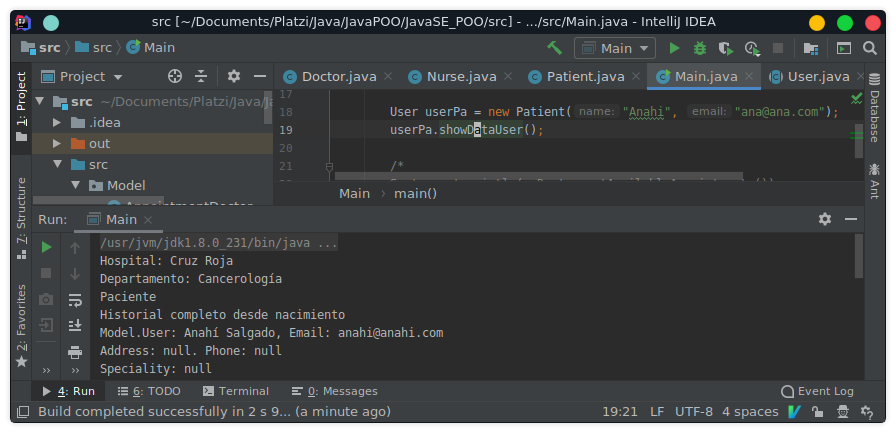
\includegraphics[scale=0.5]{./Pictures/050_polimorfismo_abstracto.png}
\end{figure}


%% Clase 28
\section{Clases Anónimas}%
Las Clases Anónimas son una forma de instanciar clases abstractas sin necesidad
de usar sus clases hijas. Pero este tipo de instanciación tiene algunas
restricciones: el ciclo de vida de estas instancias NO es duradero, no las
tendremos disponibles durante toda la ejecución del programa.


\textbf{Main.java}
\begin{minted}{java}
  import Model.Doctor;
  import Model.Patient;
  import Model.User;

  import java.util.Date;

  public class Main {
      public static void main(String[] args) {

          Doctor myDoctor = new Doctor("Anahí Salgado", "anahi@anahi.com");
          myDoctor.addAvailableAppointment(new Date(), "4pm");
          myDoctor.addAvailableAppointment(new Date(), "10pm");
          myDoctor.addAvailableAppointment(new Date(), "1pm");

          User user = new Doctor("Anahi", "ana@ana.com");
          user.showDataUser();

          User userPa = new Patient("Anahi", "ana@ana.com");
          userPa.showDataUser();

          User user1 = new User("Anahi", "ana@ana.com") {
              @Override
              public void showDataUser() {
                  System.out.println("Doctor\n");
                  System.out.println("Hospital: Cruz Verde");
                  System.out.println("Departamento: Geriatría");
              }
          };
          user1.showDataUser();

          /*
          System.out.println(myDoctor.getAvailableAppointments());

          for (Model.Doctor.AvailableAppointment aA: myDoctor.getAvailableAppointments()) {
              System.out.println(aA.getDate() + " " + aA.getTime());
          }
          */

          System.out.println(myDoctor);

          System.out.println();
          System.out.println();
          Patient patient = new Patient("Alejandra", "alejandra@mail.com");
          System.out.println(patient);
      }
  }
\end{minted}

\begin{figure}[h!]
  \centering
  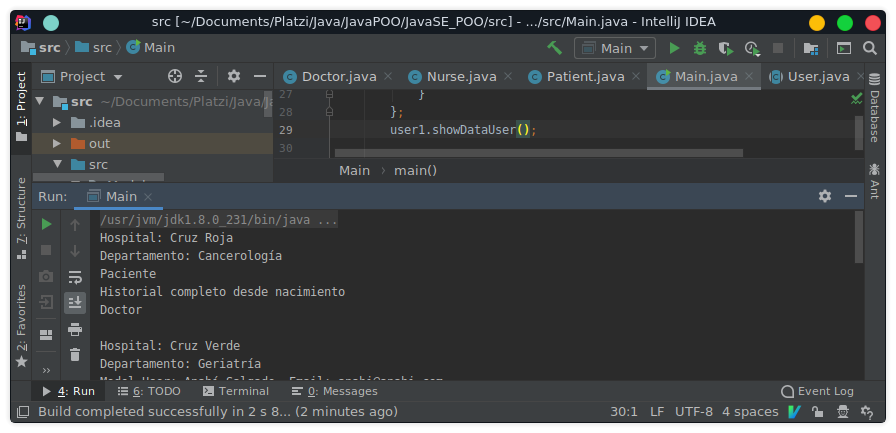
\includegraphics[scale=0.5]{./Pictures/051_clase_anonima.png}
\end{figure}



%% Clase 29
\section{Diferencias entre las Interfaces y las Clases Abstractas}%


%% Clase 30
\section{Interfaces en Java 8 y 9}%
Las Interfaces nos permiten usar métodos abstractos y campos constantes para
implementar herencia/polimorfismo de forma muy similar a las clases
abstractas.\\

A partir de Java 8 podemos tener implementación en métodos para heredar y
reutilizar diferentes comportamientos. No todos los métodos de nuestras
interfaces deben ser abstractos, ahora podemos usar el modificador de acceso
default y desde Java 9 también private.\\

Recuerda que el nivel de acceso de default y private son los mismos que
estudiamos en clases anteriores.\\

\begin{minted}{java}
  public interface MyInterface {
    // Métodos default: nos permite heredar la definición
    // de la función y también su implementación...
    default void defaultMethod() {
      privateMethod("Hello from the default method!");
    }

    // Métodos private: nos permiten definir comportamiento,
    // pero solo se puede usar desde otras clases de esta
    // interfaz, no se hereda a la clase hija....
    private void privateMethod(final String message) {
      System.out.println(message);
    }

    // Métodos abstractos: recuerda que todos los métodos
    // son abstractos por defecto...
    void normalMethod();
  }
\end{minted}



%% Clase 31
\section{Herencia en interfaces}%
Las interfaces pueden heredar de otras interfaces utilizando la palabra clave
extends, el concepto de herencia se aplicará como naturalmente se practica en
clases, es decir, la interfaz heredará y adquirirá los métodos de la interfaz
padre.\\

Una cosa interesante que sucede en caso de herencia con interfaces es que, aquí
sí es permitido la herencia múltiple como ves a continuación:\\

\begin{minted}{java}
  public interface IReadable {
    public void read();
  }

  public interface Visualizable extends IReadable, Serializable {
    public void setViewed();
    public Boolean isViewed();
    public String timeViewed();
  }
\end{minted}

Además siguiendo las implementaciones de métodos default y private de las
versiones Java 8 y 9 respectivamente podemos sobreescribir métodos y añadirles
comportamiento, si es el caso.\\

\begin{minted}{java}
  public interface Visualizable extends IReadable, Serializable {
    public void setViewed();
    public Boolean isViewed();
    public String timeViewed();
    @Override
    default void read() {
      // TODO Auto-generated method stub
    }
  }
\end{minted}


%% Clase 32
\section{Simulando autenticación de usuarios}%
En este momento la capa de modelo que maneja los objetos, vamos a unirla con la
capa de User Interface.\\

\textbf{ui/UIMenu.java}
\begin{minted}{java}
  package ui;

  import Model.Doctor;
  import Model.Patient;

  import java.util.ArrayList;
  import java.util.Scanner;

  public class UIMenu {

      public static final String[] MONTHS = {
          "Enero", "Febrero", "Marzo", "Abril", "Mayo", "Junio",
          "Julio", "Agosto", "Setiembre", "Octubre", "Noviembre", "Diciembre"
      };
      public static Doctor doctorLogged;
      public static Patient patientLogged;

      public static void showMenu() {
          System.out.println("Welcome to My Appointments");
          System.out.println("Selecciona la acción deseada");

          int response = 0;
          do {
              System.out.println("1. Doctor");
              System.out.println("2. Patient");
              System.out.println("0. Salir");

              Scanner sc = new Scanner(System.in);
              response = Integer.valueOf(sc.nextLine());


              switch (response) {
                  case 1:
                      response = 0;
                      System.out.println("Doctor");
                      authUser(1);
                      break;
                  case 2:
                      response = 0;
                      authUser(2);
                      break;
                  case 0:
                      System.out.println("Thank you for you visit.");
                      break;
                  default:
                      System.out.println("Please select a correct answer.");
              }
          } while (response != 0);
      }

      private static void authUser(int userType) {
          // userType = 1 Doctor
          // userType = 2 Paciente

          ArrayList<Doctor> doctors = new ArrayList<>();
          doctors.add(new Doctor("Alejandro Martinez", "alejandro@mail.com"));
          doctors.add(new Doctor("Karen Sosa", "karen@mail.com"));
          doctors.add(new Doctor("Rocío Gómez", "rocio@mail.com"));

          ArrayList<Patient> patients = new ArrayList<>();
          patients.add(new Patient("Anahí Salgado", "anahi@mail.com"));
          patients.add(new Patient("Roberto Rodríguez", "roberto@mail.com"));
          patients.add(new Patient("Carlos Sánchez", "carlos@mail.com"));

          boolean emailCorrect = false;

          do {
              System.out.println("Insert your email: [a@a.com] ");
              Scanner sc = new Scanner(System.in);
              String email = sc.nextLine();
              if (userType == 1) {
                  for (Doctor d: doctors) {
                      if (d.getEmail().equals(email)) {
                          emailCorrect = true;
                          // Obtener el usuario logeado
                          doctorLogged = d;
                          // ShowDoctorMenu
                      }
                  }
              }

              if (userType == 2) {
                  for (Patient p: patients) {
                      if (p.getEmail().equals(email)) {
                          emailCorrect = true;
                          // Obtener el usuario logeado
                          patientLogged = p;
                          // ShowPatientMenu
                      }
                  }
              }
          } while (!emailCorrect);
      }

      public static void showPatientMenu() {
          int response = 0;
          do {
              System.out.println("\n\n");
              System.out.println("Model.Patient");
              System.out.println("1. Book an appointment");
              System.out.println("2. My appointments");
              System.out.println("0. Return");

              Scanner sc = new Scanner(System.in);
              response = Integer.valueOf(sc.nextLine());

              switch (response) {
                  case 1:
                      System.out.println("::Book an appointment");
                      for (int i = 0; i < 3; i++) {
                          System.out.println(i + ". " + MONTHS[i]);
                      }
                      break;
                  case 2:
                      System.out.println("::My appointments");
                      break;
                  case 0:
                      showMenu();
                      break;
              }
          } while (response != 0);
      }
  }
\end{minted}



%% Clase 33
\section{Modularizando la UI de Doctores}%
Acabamos de hacer la simulación de la autenticación de un usuario. Ahora vamos
a modularizar nuestra interfaz de usuario.\\

\textbf{ui/UIDoctorMenu.java}
\begin{minted}{java}
  package ui;

  import java.util.Scanner;

  public class UIDoctorMenu {
      public static void showDoctorMenu() {
          int response = 0;
          do {
              System.out.println("\n\n");
              System.out.println("Doctor");
              System.out.println("Welcome " + UIMenu.doctorLogged.getName());
              System.out.println("1. Add Available Appointment");
              System.out.println("2. My Schedule Appointment");
              System.out.println("0. Logout");

              Scanner sc = new Scanner(System.in);
              response = Integer.valueOf(sc.nextLine());

              switch ( response ) {
                  case 1:
                      break;
                  case 2:
                      break;
                  case 0:
                      UIMenu.showMenu();
                      break;
              }
          } while (response != 0)
      }

      private static void showAddAvailableAppointmentsMenu() {
          int response = 0;
          do {
              System.out.println();
              System.out.println("::Add Available Appointment");
              System.out.println(":: Select a Month");

              for (int i = 0; i < 3; i++) {
                  int j = i + 1;
                  System.out.println(j + ". " + UIMenu.MONTHS[i]);
              }
              System.out.println("0. Return");

              Scanner sc = new Scanner(System.in);
              response = Integer.valueOf(sc.nextLine());

              if (response > 0 && response < 4) {
                  // 1, 2, 3
                  int monthSelected = response;
                  System.out.println(monthSelected + " . " + UIMenu.MONTHS[monthSelected]);

                  System.out.println("Insert the date available: [dd/mm/yy] ");
                  String date = sc.nextLine();

                  System.out.println("You date is: " + date + "\n1. Correct \n2. Change Date");
              } else if (response == 0) {
                  showDoctorMenu();
              }
          } while( response != 0 );
      }
  }
\end{minted}



%% Clase 34
\section{Definiendo las citas disponibles}%
Algunas veces necesitamos trabajar las fechas como tipo de dato Date y otras
veces como String. Para resolver esto podemos usar SimpleDateFormat.\\

\begin{minted}{java}
  SimpleDateFormat format = new SimpleDateFormat(pattern: "dd/MM/yyyy");

  // Transformar fechas de formato String a Date:
  this.date = format.parse(dateAsString);

  // Transformar fechas de formato Date a String:
  this.date = format.format(dateAsDate);
\end{minted}


\textbf{ui/UIDoctorMenu.java}
\begin{minted}{java}
  package ui;

  import Model.Doctor;

  import java.util.ArrayList;
  import java.util.Scanner;

  public class UIDoctorMenu {

      public static ArrayList<Doctor> doctorsAvailableAppointments = new ArrayList<>();

      public static void showDoctorMenu() {
          int response = 0;
          do {
              System.out.println("\n\n");
              System.out.println("Doctor");
              System.out.println("Welcome " + UIMenu.doctorLogged.getName());
              System.out.println("1. Add Available Appointment");
              System.out.println("2. My Schedule Appointment");
              System.out.println("0. Logout");

              Scanner sc = new Scanner(System.in);
              response = Integer.valueOf(sc.nextLine());

              switch ( response ) {
                  case 1:
                      break;
                  case 2:
                      break;
                  case 0:
                      UIMenu.showMenu();
                      break;
              }
          } while (response != 0);
      }

      private static void showAddAvailableAppointmentsMenu() {
          int response = 0;
          do {
              System.out.println();
              System.out.println("::Add Available Appointment");
              System.out.println(":: Select a Month");

              for (int i = 0; i < 3; i++) {
                  int j = i + 1;
                  System.out.println(j + ". " + UIMenu.MONTHS[i]);
              }
              System.out.println("0. Return");

              Scanner sc = new Scanner(System.in);
              response = Integer.valueOf(sc.nextLine());

              if (response > 0 && response < 4) {
                  // 1, 2, 3
                  int monthSelected = response;
                  System.out.println(monthSelected + " . " + UIMenu.MONTHS[monthSelected]);

                  System.out.println("Insert the date available: [dd/mm/yy] ");
                  String date = sc.nextLine();

                  System.out.println("You date is: " + date + "\n1. Correct \n2. Change Date");
                  int responseDate = Integer.valueOf(sc.nextLine());
                  if (responseDate == 2) continue;

                  int responseTime = 0;
                  String time = "";
                  do {
                      System.out.println("Insert the time available for date: " + date + " [16:00] ");
                      time = sc.nextLine();
                      System.out.println("Your time is: " + time + "\n1. Correct \n2. Change Time");
                      responseTime = Integer.valueOf(sc.nextLine());
                  } while (responseTime == 2);

                  UIMenu.doctorLogged.addAvailableAppointment(date, time);
                  checkDoctorAvailableAppointments(UIMenu.doctorLogged);
              } else if (response == 0) {
                  showDoctorMenu();
              }
          } while( response != 0 );
      }

      private static void checkDoctorAvailableAppointments (Doctor doctor) {
          if (doctor.getAvailableAppointments().size() > 0
              && !doctorsAvailableAppointments.contains(doctor)) {
              doctorsAvailableAppointments.add(doctor);
          }
      }
  }
\end{minted}

\textbf{ui/UIMenu.java}
\begin{minted}{java}
  package ui;

  import Model.Doctor;
  import Model.Patient;

  import java.util.ArrayList;
  import java.util.Scanner;

  public class UIMenu {

      public static final String[] MONTHS = {
          "Enero", "Febrero", "Marzo", "Abril", "Mayo", "Junio",
          "Julio", "Agosto", "Setiembre", "Octubre", "Noviembre", "Diciembre"
      };
      public static Doctor doctorLogged;
      public static Patient patientLogged;

      public static void showMenu() {
          System.out.println("Welcome to My Appointments");
          System.out.println("Selecciona la acción deseada");

          int response = 0;
          do {
              System.out.println("1. Doctor");
              System.out.println("2. Patient");
              System.out.println("0. Salir");

              Scanner sc = new Scanner(System.in);
              response = Integer.valueOf(sc.nextLine());


              switch (response) {
                  case 1:
                      response = 0;
                      System.out.println("Doctor");
                      authUser(1);
                      break;
                  case 2:
                      response = 0;
                      authUser(2);
                      break;
                  case 0:
                      System.out.println("Thank you for you visit.");
                      break;
                  default:
                      System.out.println("Please select a correct answer.");
              }
          } while (response != 0);
      }

      private static void authUser(int userType) {
          // userType = 1 Doctor
          // userType = 2 Paciente

          ArrayList<Doctor> doctors = new ArrayList<>();
          doctors.add(new Doctor("Alejandro Martinez", "alejandro@mail.com"));
          doctors.add(new Doctor("Karen Sosa", "karen@mail.com"));
          doctors.add(new Doctor("Rocío Gómez", "rocio@mail.com"));

          ArrayList<Patient> patients = new ArrayList<>();
          patients.add(new Patient("Anahí Salgado", "anahi@mail.com"));
          patients.add(new Patient("Roberto Rodríguez", "roberto@mail.com"));
          patients.add(new Patient("Carlos Sánchez", "carlos@mail.com"));

          boolean emailCorrect = false;

          do {
              System.out.println("Insert your email: [a@a.com] ");
              Scanner sc = new Scanner(System.in);
              String email = sc.nextLine();
              if (userType == 1) {
                  for (Doctor d: doctors) {
                      if (d.getEmail().equals(email)) {
                          emailCorrect = true;
                          // Obtener el usuario logeado
                          doctorLogged = d;
                          // ShowDoctorMenu
                      }
                  }
              }

              if (userType == 2) {
                  for (Patient p: patients) {
                      if (p.getEmail().equals(email)) {
                          emailCorrect = true;
                          // Obtener el usuario logeado
                          patientLogged = p;
                          // ShowPatientMenu
                      }
                  }
              }
          } while (!emailCorrect);
      }

      public static void showPatientMenu() {
          int response = 0;
          do {
              System.out.println("\n\n");
              System.out.println("Model.Patient");
              System.out.println("1. Book an appointment");
              System.out.println("2. My appointments");
              System.out.println("0. Return");

              Scanner sc = new Scanner(System.in);
              response = Integer.valueOf(sc.nextLine());

              switch (response) {
                  case 1:
                      System.out.println("::Book an appointment");
                      for (int i = 0; i < 3; i++) {
                          System.out.println(i + ". " + MONTHS[i]);
                      }
                      break;
                  case 2:
                      System.out.println("::My appointments");
                      break;
                  case 0:
                      showMenu();
                      break;
              }
          } while (response != 0);
      }
  }
\end{minted}

\textbf{Model/Doctor.java}
\begin{minted}{java}
  package Model;

  import java.text.ParseException;
  import java.text.SimpleDateFormat;
  import java.util.ArrayList;
  import java.util.Date;

  public class Doctor extends User {
      // Atributo
      private String speciality;

      public Doctor(String name, String email) {
          super(name, email);
      }

      public String getSpeciality() {
          return speciality;
      }

      public void setSpeciality(String speciality) {
          this.speciality = speciality;
      }

      public void setAvailableAppointments(ArrayList<AvailableAppointment> availableAppointments) {
          this.availableAppointments = availableAppointments;
      }

      ArrayList<AvailableAppointment> availableAppointments = new ArrayList<>();
      public void addAvailableAppointment(String date, String time) {

          availableAppointments.add(new Doctor.AvailableAppointment(date, time));
      }

      public ArrayList<AvailableAppointment> getAvailableAppointments() {
          return availableAppointments;
      }

      @Override
      public String toString() {
          return super.toString() + "\nSpeciality: " + speciality +
          "\nAvailable: " + availableAppointments.toString();
      }

      @Override
      public void showDataUser() {
          System.out.println("Hospital: Cruz Roja");
          System.out.println("Departamento: Cancerología");
      }

      public static class AvailableAppointment {
          private int id;
          private Date date;
          private String time;
          SimpleDateFormat format = new SimpleDateFormat("dd/MM/yyyy");

          public AvailableAppointment(String date, String time) {
              try {
                  this.date = format.parse(date);
              } catch (ParseException e) {
                  e.printStackTrace();
              }
              this.time = time;
          }

          public Date getDate() {
              return date;
          }

          public String getDate(String DATE) {
              return format.format(date);
          }

          public void setDate(Date date) {
              this.date = date;
          }

          public String getTime() {
              return time;
          }

          public void setTime(String time) {
              this.time = time;
          }

          @Override
          public String toString() {
              return "Available Appointments \nDate: " + date + "\nTime: " + time;
          }
      }
  }
\end{minted}


%% Clase 35
\section{Modularizando la UI de Pacientes}%
Antes de correr nuestro proyecto, vamos a agregar los menus que acabamos de
crear.\\

\textbf{ui/UIMenu.java}
\begin{minted}{java}
  package ui;

  import Model.Doctor;
  import Model.Patient;

  import java.util.ArrayList;
  import java.util.Scanner;

  public class UIMenu {

      public static final String[] MONTHS = {
          "Enero", "Febrero", "Marzo", "Abril", "Mayo", "Junio",
          "Julio", "Agosto", "Setiembre", "Octubre", "Noviembre", "Diciembre"
      };
      public static Doctor doctorLogged;
      public static Patient patientLogged;

      public static void showMenu() {
          System.out.println("Welcome to My Appointments");
          System.out.println("Selecciona la acción deseada");

          int response = 0;
          do {
              System.out.println("1. Doctor");
              System.out.println("2. Patient");
              System.out.println("0. Salir");

              Scanner sc = new Scanner(System.in);
              response = Integer.valueOf(sc.nextLine());


              switch (response) {
                  case 1:
                      response = 0;
                      System.out.println("Doctor");
                      authUser(1);
                      break;
                  case 2:
                      response = 0;
                      authUser(2);
                      break;
                  case 0:
                      System.out.println("Thank you for you visit.");
                      break;
                  default:
                      System.out.println("Please select a correct answer.");
              }
          } while (response != 0);
      }

      private static void authUser(int userType) {
          // userType = 1 Doctor
          // userType = 2 Paciente

          ArrayList<Doctor> doctors = new ArrayList<>();
          doctors.add(new Doctor("Alejandro Martinez", "alejandro@mail.com"));
          doctors.add(new Doctor("Karen Sosa", "karen@mail.com"));
          doctors.add(new Doctor("Rocío Gómez", "rocio@mail.com"));

          ArrayList<Patient> patients = new ArrayList<>();
          patients.add(new Patient("Anahí Salgado", "anahi@mail.com"));
          patients.add(new Patient("Roberto Rodríguez", "roberto@mail.com"));
          patients.add(new Patient("Carlos Sánchez", "carlos@mail.com"));

          boolean emailCorrect = false;

          do {
              System.out.println("Insert your email: [a@a.com] ");
              Scanner sc = new Scanner(System.in);
              String email = sc.nextLine();
              if (userType == 1) {
                  for (Doctor d: doctors) {
                      if (d.getEmail().equals(email)) {
                          emailCorrect = true;
                          // Obtener el usuario logeado
                          doctorLogged = d;
                          UIDoctorMenu.showDoctorMenu();
                      }
                  }
              }

              if (userType == 2) {
                  for (Patient p: patients) {
                      if (p.getEmail().equals(email)) {
                          emailCorrect = true;
                          // Obtener el usuario logeado
                          patientLogged = p;
                          // ShowPatientMenu
                      }
                  }
              }
          } while (!emailCorrect);
      }

      public static void showPatientMenu() {
          int response = 0;
          do {
              System.out.println("\n\n");
              System.out.println("Model.Patient");
              System.out.println("1. Book an appointment");
              System.out.println("2. My appointments");
              System.out.println("0. Return");

              Scanner sc = new Scanner(System.in);
              response = Integer.valueOf(sc.nextLine());

              switch (response) {
                  case 1:
                      System.out.println("::Book an appointment");
                      for (int i = 0; i < 3; i++) {
                          System.out.println(i + ". " + MONTHS[i]);
                      }
                      break;
                  case 2:
                      System.out.println("::My appointments");
                      break;
                  case 0:
                      showMenu();
                      break;
              }
          } while (response != 0);
      }
  }
\end{minted}

\textbf{ui/UIDoctorMenu.java}
\begin{minted}{java}
  package ui;

  import Model.Doctor;

  import java.util.ArrayList;
  import java.util.Scanner;

  public class UIDoctorMenu {

      public static ArrayList<Doctor> doctorsAvailableAppointments = new ArrayList<>();

      public static void showDoctorMenu() {
          int response = 0;
          do {
              System.out.println("\n\n");
              System.out.println("Doctor");
              System.out.println("Welcome " + UIMenu.doctorLogged.getName());
              System.out.println("1. Add Available Appointment");
              System.out.println("2. My Schedule Appointment");
              System.out.println("0. Logout");

              Scanner sc = new Scanner(System.in);
              response = Integer.valueOf(sc.nextLine());

              switch ( response ) {
                  case 1:
                      showAddAvailableAppointmentsMenu();
                      break;
                  case 2:
                      break;
                  case 0:
                      UIMenu.showMenu();
                      break;
              }
          } while (response != 0);
      }

      private static void showAddAvailableAppointmentsMenu() {
          int response = 0;
          do {
              System.out.println();
              System.out.println("::Add Available Appointment");
              System.out.println(":: Select a Month");

              for (int i = 0; i < 3; i++) {
                  int j = i + 1;
                  System.out.println(j + ". " + UIMenu.MONTHS[i]);
              }
              System.out.println("0. Return");

              Scanner sc = new Scanner(System.in);
              response = Integer.valueOf(sc.nextLine());

              if (response > 0 && response < 4) {
                  // 1, 2, 3
                  int monthSelected = response;
                  System.out.println(monthSelected + " . " + UIMenu.MONTHS[monthSelected-1]);

                  System.out.println("Insert the date available: [dd/mm/yy] ");
                  String date = sc.nextLine();

                  System.out.println("You date is: " + date + "\n1. Correct \n2. Change Date");
                  int responseDate = Integer.valueOf(sc.nextLine());
                  if (responseDate == 2) continue;

                  int responseTime = 0;
                  String time = "";
                  do {
                      System.out.println("Insert the time available for date: " + date + " [16:00] ");
                      time = sc.nextLine();
                      System.out.println("Your time is: " + time + "\n1. Correct \n2. Change Time");
                      responseTime = Integer.valueOf(sc.nextLine());
                  } while (responseTime == 2);

                  UIMenu.doctorLogged.addAvailableAppointment(date, time);
                  checkDoctorAvailableAppointments(UIMenu.doctorLogged);
              } else if (response == 0) {
                  showDoctorMenu();
              }
          } while( response != 0 );
      }

      private static void checkDoctorAvailableAppointments (Doctor doctor) {
          if (doctor.getAvailableAppointments().size() > 0
              && !doctorsAvailableAppointments.contains(doctor)) {
              doctorsAvailableAppointments.add(doctor);
          }
      }
  }
\end{minted}

\textbf{Main.java}
\begin{minted}{java}
  import static ui.UIMenu.showMenu;

  public class Main {
      public static void main(String[] args) {
          showMenu();
      }
  }
\end{minted}

\begin{figure}[h!]
  \centering
  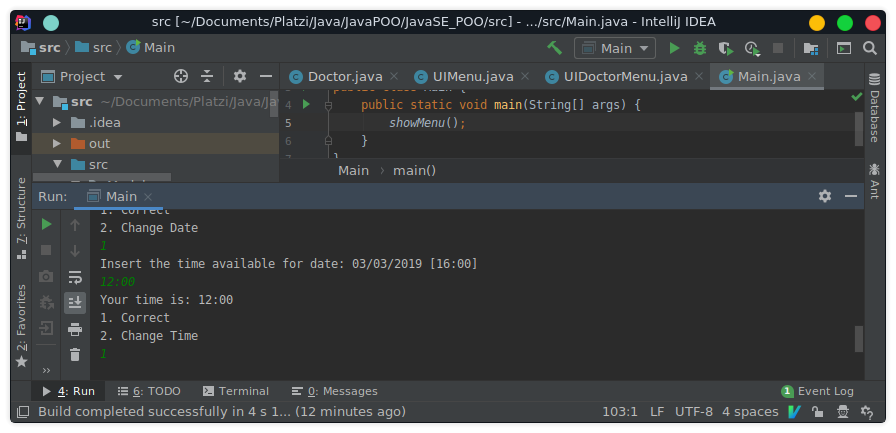
\includegraphics[scale=0.5]{./Pictures/052_uidoctor_funcional.png}
\end{figure}


Ahora vamos a empezar a trabajar con el interfaz de usuario para Patient.\\

\textbf{ui/UIPatientMenu.java}
\begin{minted}{java}
  package ui;

  import java.util.Scanner;

  public class UIPatientMenu {

      public static void showPatientMenu() {
          int response = 0;
          do {
              System.out.println("\n\n");
              System.out.println("Patient");
              System.out.println("Welcome: " + UIMenu.patientLogged);
              System.out.println("1. Book an appointment");
              System.out.println("2. My Appointments");
              System.out.println("0. Logout");

              Scanner sc = new Scanner(System.in);
              response = Integer.valueOf(sc.nextLine());

              switch (response) {
                  case 1:
                      break;
                  case 2:
                      break;
                  case 0:
                      UIMenu.showMenu();
                      break;
              }
          } while (response != 0);
      }

      private static void showBookAppointmentMenu() {
          int response = 0;
          do {
              System.out.println("::Book an appointment");
              System.out.println(":: Select date: ");
          } while (response != 0);
      }

  }
\end{minted}


%% Clase 36
\section{Recorriendo estructuras de árbol en Java}%
Las estructuras de árbol pertenecen al grupo de estructuras de datos no
lineales, es decir, donde toda la información es almacenada con un orden
específico. En estas estructuras tenemos “troncos” principales con diferentes
ramificaciones que surgen a partir de ellos. Son muy útiles para trabajar con
grandes cantidades de datos organizados de forma jerárquica.\\

La forma de implementarlos en Java es usando un Map de tipo TreeMap. Recuerda
que también podemos guardar Maps dentro de otros Maps. De esta forma podemos
definir una lista ordenada de doctores y sus fechas disponibles para agendar
citas médicas.\\

\begin{minted}{java}
  // 1. Doctor#1
  // - - - Fecha#1
  // - - - Fecha#2
  // 2. Doctor#2
  // - - - Fecha#1
  // - - - Fecha#2
  // 3. Doctor#3
  // - - - Fecha#1
  // - - - Fecha#2
  Map<Integer, Map<Integer, Doctor>> doctors = new TreeMap<>();
\end{minted}

\textbf{ui/UIPatientMenu.java}
\begin{minted}{java}
  package ui;

  import Model.Doctor;

  import java.util.ArrayList;
  import java.util.Map;
  import java.util.Scanner;
  import java.util.TreeMap;

  public class UIPatientMenu {

      public static void showPatientMenu() {
          int response = 0;
          do {
              System.out.println("\n\n");
              System.out.println("Patient");
              System.out.println("Welcome: " + UIMenu.patientLogged);
              System.out.println("1. Book an appointment");
              System.out.println("2. My Appointments");
              System.out.println("0. Logout");

              Scanner sc = new Scanner(System.in);
              response = Integer.valueOf(sc.nextLine());

              switch (response) {
                  case 1:
                      break;
                  case 2:
                      break;
                  case 0:
                      UIMenu.showMenu();
                      break;
              }
          } while (response != 0);
      }

      private static void showBookAppointmentMenu() {
          int response = 0;
          do {
              System.out.println("::Book an appointment");
              System.out.println(":: Select date: ");
              // Numeracion de la lista de fechas
              // Indice de la fecha seleccionada
              // [doctors]
              // 1.- doctor 1
                      // - 1 fecha 1
                      // - 2 fecha 2
              // 2.- doctor 2
              // 3.- doctor 3
              Map<Integer, Map<Integer, Doctor>> doctors = new TreeMap<>();
              int k=0;
              for (int i=1; i<UIDoctorMenu.doctorsAvailableAppointments.size(); i++) {
                  ArrayList<Doctor.AvailableAppointment> availableAppointments
                          = UIDoctorMenu.doctorsAvailableAppointments.get(i).getAvailableAppointments();

                  Map<Integer, Doctor> doctorAppointments = new TreeMap<>();

                  for (int j = 0; j < availableAppointments.size(); j++) {
                      k++;
                      System.out.println(k + ". " + availableAppointments.get(j).getDate());
                      doctorAppointments.put(Integer.valueOf(j), UIDoctorMenu.doctorsAvailableAppointments.get(i));
                      doctors.put(Integer.valueOf(k), doctorAppointments);
                  }
              }

              Scanner sc = new Scanner(System.in);
              int responseDateSelected = Integer.valueOf(sc.nextLine());

          } while (response != 0);
      }

  }
\end{minted}


\textbf{Model/Doctor.java}
\begin{minted}{java}
  package Model;

  import java.text.ParseException;
  import java.text.SimpleDateFormat;
  import java.util.ArrayList;
  import java.util.Date;

  public class Doctor extends User {
      // Atributo
      private String speciality;
      private ArrayList<AvailableAppointment> availableAppointments = new ArrayList<>();

      public Doctor(String name, String email) {
          super(name, email);
      }

      public String getSpeciality() {
          return speciality;
      }

      public void setSpeciality(String speciality) {
          this.speciality = speciality;
      }

      public void setAvailableAppointments(ArrayList<AvailableAppointment> availableAppointments) {
          this.availableAppointments = availableAppointments;
      }

      public void addAvailableAppointment(String date, String time) {

          availableAppointments.add(new Doctor.AvailableAppointment(date, time));
      }

      public ArrayList<AvailableAppointment> getAvailableAppointments() {
          return availableAppointments;
      }

      @Override
      public String toString() {
          return super.toString() + "\nSpeciality: " + speciality +
          "\nAvailable: " + availableAppointments.toString();
      }

      @Override
      public void showDataUser() {
          System.out.println("Hospital: Cruz Roja");
          System.out.println("Departamento: Cancerología");
      }

      public static class AvailableAppointment {
          private int id;
          private Date date;
          private String time;
          SimpleDateFormat format = new SimpleDateFormat("dd/MM/yyyy");

          public AvailableAppointment(String date, String time) {
              try {
                  this.date = format.parse(date);
              } catch (ParseException e) {
                  e.printStackTrace();
              }
              this.time = time;
          }

          public Date getDate(String DATE) {
              return date;
          }

          public String getDate() {
              return format.format(date);
          }

          public void setDate(Date date) {
              this.date = date;
          }

          public String getTime() {
              return time;
          }

          public void setTime(String time) {
              this.time = time;
          }

          @Override
          public String toString() {
              return "Available Appointments \nDate: " + date + "\nTime: " + time;
          }
      }
  }
\end{minted}


%% Clase 37
\section{Agendando Citas}%

\textbf{ui/UIPatientMenu.java}
\begin{minted}{java}
  package ui;

  import Model.Doctor;

  import java.util.ArrayList;
  import java.util.Map;
  import java.util.Scanner;
  import java.util.TreeMap;

  public class UIPatientMenu {

      public static void showPatientMenu() {
          int response = 0;
          do {
              System.out.println("\n\n");
              System.out.println("Patient");
              System.out.println("Welcome: " + UIMenu.patientLogged);
              System.out.println("1. Book an appointment");
              System.out.println("2. My Appointments");
              System.out.println("0. Logout");

              Scanner sc = new Scanner(System.in);
              response = Integer.valueOf(sc.nextLine());

              switch (response) {
                  case 1:
                      showBookAppointmentMenu();
                      break;
                  case 2:
                      break;
                  case 0:
                      UIMenu.showMenu();
                      break;
              }
          } while (response != 0);
      }

      private static void showBookAppointmentMenu() {
          int response = 0;
          do {
              System.out.println("::Book an appointment");
              System.out.println(":: Select date: ");
              // Numeracion de la lista de fechas
              // Indice de la fecha seleccionada
              // [doctors]
              // 1.- doctor 1
                      // - 1 fecha 1
                      // - 2 fecha 2
              // 2.- doctor 2
              // 3.- doctor 3
              Map<Integer, Map<Integer, Doctor>> doctors = new TreeMap<>();
              int k=0;
              for (int i=1; i<UIDoctorMenu.doctorsAvailableAppointments.size(); i++) {
                  ArrayList<Doctor.AvailableAppointment> availableAppointments
                          = UIDoctorMenu.doctorsAvailableAppointments.get(i).getAvailableAppointments();

                  Map<Integer, Doctor> doctorAppointments = new TreeMap<>();

                  for (int j = 0; j < availableAppointments.size(); j++) {
                      k++;
                      System.out.println(k + ". " + availableAppointments.get(j).getDate());
                      doctorAppointments.put(Integer.valueOf(j), UIDoctorMenu.doctorsAvailableAppointments.get(i));
                      doctors.put(Integer.valueOf(k), doctorAppointments);
                  }
              }

              Scanner sc = new Scanner(System.in);
              int responseDateSelected = Integer.valueOf(sc.nextLine());
              Map<Integer, Doctor> doctorAvailableSelected = doctors.get(responseDateSelected);
              Integer indexDate = 0;
              Doctor doctorSelected = new Doctor("", "");

              for (Map.Entry<Integer, Doctor> doc :doctorAvailableSelected.entrySet()) {
                  indexDate = doc.getKey();
                  doctorSelected = doc.getValue();
              }

              System.out.println(doctorSelected.getName() +
                      ". Date: " + doctorSelected.getAvailableAppointments().get(indexDate).getDate() +
                      ". Time: " + doctorSelected.getAvailableAppointments().get(indexDate).getTime());

              System.out.println("Confirm your appointment: \n1. Yes \n2. Change Data");
              response = Integer.valueOf(sc.nextLine());

              if (response == 1) {
                  UIMenu.patientLogged.addAppointmentDoctors(
                          doctorSelected,
                          doctorSelected.getAvailableAppointments().get(indexDate).getDate(null),
                          doctorSelected.getAvailableAppointments().get(indexDate).getTime());

                  showPatientMenu();
              }
          } while (response != 0);
      }

      private static void showPatientMyAppointments() {
          int response = 0;
          do {
              System.out.println("::My Appointments");
              if (UIMenu.patientLogged.getAppointmentDoctors().size() == 0) {
                  System.out.println("Don't have appointments");
                  break;
              }

              for (int i = 0; i < UIMenu.patientLogged.getAppointmentDoctors().size(); i++) {
                  int j = i + 1;
                  System.out.println(j + ". " +
                          "Date: " + UIMenu.patientLogged.getAppointmentDoctors().get(i).getDate() +
                          " Time: " + UIMenu.patientLogged.getAppointmentDoctors().get(i).getTime() +
                          "\n Doctor: " + UIMenu.patientLogged.getAppointmentDoctors().get(i).getDoctor().getName());
              }

              System.out.println("0. Return");
          } while (response != 0);
      }
  }
\end{minted}


%% Clase 38
\section{Cierre del curso: Continúa con Programación Funcional en Java}%
¡Felicitaciones por terminar el Curso de Introducción a Java SE!

En este curso aprendimos a implementar los 4 pilares de la programación
orientada a objetos en Java con un proyecto para agendar citas médicas.

Recuerda resolver los ejercicios, completar el examen, darle 5 estrellas a la
profesora y compartir tu proyecto, notas, dudas y comentarios en la sección de
discusiones.

No olvides que puedes continuar tu ruta de aprendizaje de Java con los
siguientes cursos:

\begin{itemize}
  \item Curso de Java SE: Programación Funcional
  \item Curso de Java SE: Persistencia de Datos
\end{itemize}



































\vspace{2cm}
\LARGE\textit{RuneCode}


\end{document}

